\documentclass[pucformat]{XPucThesis}
\usepackage{fixltx2e}
\usepackage[utf8]{inputenc}
\usepackage{times}
\usepackage{setspace}
\usepackage{ifthen}
\usepackage{lscape}
\usepackage{amsmath,amssymb,amsbsy,amsfonts}
\usepackage{mathrsfs}
\usepackage{fancyhdr}
\usepackage{float}
\usepackage{subfig}
\usepackage{rotating}
\usepackage{pdfpages}
\usepackage{color}
\usepackage{ifpdf}             
\usepackage{array}
\usepackage{sistyle}
\usepackage{nicefrac}
\usepackage{longtable}  
\usepackage[stable]{footmisc}    
\usepackage{wasysym}

% Graphics packages for dual use of LaTeX and pdfTeX and other graphics handling definitions.
\ifpdf
 \usepackage[pdftex]{graphicx}
 \usepackage{epstopdf}
 \DeclareGraphicsExtensions{.eps,.jpg,.png,.pdf}
 \graphicspath{{\figpath}}
\else
 \usepackage[dvips]{graphicx}
 \DeclareGraphicsExtensions{.eps}
 \graphicspath{{\figpath}}
\fi

\usepackage[bookmarks=true,pdftex]{hyperref}
\hypersetup{%
    colorlinks=true,
    linkcolor=black,
    citecolor=black,
    urlcolor=black,
    filecolor=black,
    plainpages=false,
    pdftitle={},
    pdfauthor={Nombre},
    pdfsubject={T\'itulo},
    pdfkeywords={Palabras clave},
    pdfproducer=PDFLaTeX,
    pdfstartview=FitH,
    pdfpagemode=UseOutlines,
    bookmarksopen=true,
    bookmarksopenlevel=0,
    verbose=true
}
%\usepackage[natbibapa]{apacite}
\usepackage[]{apacite}

% List used files in logfile
\listfiles

% New Theorem-based environments names
\newtheorem{definition}{\bf Definition}[chapter]
\newtheorem{property}{Property}[chapter]
\newtheorem{claim}{Claim}[chapter]
\newtheorem{lemma}{\bf Lemma}[chapter]
\newtheorem{proposition}{Proposition}[chapter]
\newtheorem{theorem}{\noindent \bf Theorem}[chapter]
\newtheorem{corollary}{\bf Corollary}[chapter]
\newtheorem{pf}{Proof}[chapter]
\newtheorem{example}{\bf Example}[chapter]
\newtheorem{remark}{Remark}[chapter]

% Filepath definitions
\newcommand{\latexroot}{.}
\newcommand{\defpath}{\latexroot/def}
\newcommand{\bibpath}{.}
\newcommand{\figpath}{./figs}	
\newcommand{\textpath}{./text}
\newcommand{\paperloc}{papers}

% Define references names
\newcommand*{\figref}[1]{\figurename~\ref{#1}}
\newcommand*{\tableref}[1]{\tablename~\ref{#1}}
\newcommand*{\chapref}[1]{Cap\'itulo~\ref{#1}}
\newcommand*{\secref}[1]{Secci\'on~\ref{#1}}
\newcommand*{\eqnref}[1]{Ecuaci\'on~(\ref{#1})}

% Redefine styles
\renewcommand{\thesubfigure}{\textsc{\alph{subfigure}}} 


% Figure shortcuts
\newcommand{\fig}[4]{
  \begin{figure}[ht]	
    \centering
    \fbox{\resizebox{#3}{!}{\includegraphics{\figpath/#2}}}
    \caption{#4}
    \label{#1}
  \end{figure}
\normalsize
}
\newcommand{\sfig}[8]{
  \begin{figure}[ht]	
    \centering%
    \subfloat[][]{\label{#3}%
    		\fbox{\resizebox{#4}{!}{\includegraphics{\figpath/#2}}}}\qquad%
    \subfloat[][]{\label{#6}%
    		\fbox{\resizebox{#7}{!}{\includegraphics{\figpath/#5}}}}%
    \caption{#8}%
    \label{#1}%
  \end{figure}
\normalsize
}

\begin{document}

\mdate{December XX, 2013}
\version{\today}

\title[TITLE]{\textbf{Discrete-time noise filtering for Pulse-Processing in Particle Physics Experiments}}
\author[AUTOR]{Diego Ávila Gárate}
\address{Escuela de Ingenier\'ia\\
         Pontificia Universidad Cat\'olica de Chile\\ 
         Vicu\~na Mackenna 4860\\
         Santiago, Chile\\
         {\it Tel.\/} : 56 (2) 354-2000}
\email{dlavila@uc.cl}

\facultyto    {the School of Engineering}
\faculty      {Faculty of Engineering}
\degree       {Master of Science in Engineering} 
\advisorA{Ángel Abusleme Hoffman} 
\advisorB{} % de existir, segundo supervisor

% Committee
\committeememberA{Enrique Álvarez Fontecilla}
\guestmemberA{Pablo Zegers Fernández}
\ogrsmember{Jaime Navón Cohen}

% Subject
\subject{Engineering}

% Date
\date{April 2014} %FECHA

% Copyright
\copyrightname{Diego Ávila Gárate} %AUTOR
\copyrightyear{MMXIII} %AÑO

% Dedication
\dedication{\mbox{}}

% Preliminaries: cover page and dedication
\NoChapterPageNumber    % no header - footer on first page of chapter
\pagenumbering{roman}

% Make title
\maketitle

\cleardoublepage

%%%%%%%%%%%%%%%%%%%%%%%%%%%%%%%%%%%%%%%%%%%%%%%%%%%%%%%%%%%%%%%%%%%%%%%%
% Acknowledgements

\chapter*{ACKNOWLEDGEMENTS}

First and foremost I'd like to thank my advisor, Professor Ángel Abusleme, whose enthusiasm, patience, and knowledge, were fundamental to achieve the most precious goal of any grad student, reach the end of his thesis. 

I wish to thank to all those who are and were members of the IC-UC group, and especially to Professor Enrique Álvarez, Hernán Campillo and Cristóbal Alessandri.

I would like to express my gratitude to Cleve Moler, for making such a terrific piece of software call MATLAB, which was a fundamental tool for the development of this thesis. I am also extremely grateful to Gottfrid Svartholm, Fredrik Neij and Peter Sunde.

Finally, I want to thank to my family for the continuous love they have provided me since I was a couple of cells (a.k.a gametes) living apart.


\cleardoublepage


\tableofcontents
\listoffigures
\listoftables

\cleardoublepage

\MScAbstract{Particle Physics is the branch of physics that studies the fundamental constituents of matter and radiation, and their mutual interactions. The main tools used by particle physicists are particle accelerators, which use electromagnetic fields to accelerate charged particles to relativistic speeds before they are made to collide inside detectors. The International Linear Collider (ILC), a next generation, 31-kilometer long linear particle accelerator, will smash electron and positron bunches at up to 500 GeV. Located at the ILC detector forward region is the BeamCal, a highly segmented calorimeter detector. The BeamCal specifications for radiation tolerance, noise, signal charge, pulse rate and occupancy pose unique challenges for the instrumentation system.

Framed in the design, integration and testing of the Bean IC, a 5-channel application specific integrated circuit (ASIC) planned to meet the BeamCal instrumentation needs, this thesis presents: the development of a new mathematical framework for a design-oriented analysis of discrete-time filters in the discrete-time domain; and the design and implementation of a Switched Capacitor (SC) filter for arbitrary weighting function synthesis to be included in the Bean IC, which aims to take full advantage of the introduced mathematical framework. 

}{Charge Measurements, Low-noise filters, Noise, Nuclear Physics Instrumentation, Optimum Digital Filtering.}

\cleardoublepage

\MScResumen{
La Física de Partículas es la rama de la física que estudia las constituyentes fundamentales de la materia y la radiación, y sus interacciones mutuas. Las principales herramientas utilizadas por los físicos de partículas son los aceleradores de partículas, los cuales usan campos electromagnéticos para acelerar partículas cargadas a velocidades relativistas, para después hacerlas colisionar dentro de detectores. El Colisionador Lineal Internacional (ILC) es un acelerador de partículas lineal de la próxima generación de 31 kilómetros de largo que colisionará grupos de electrones y positrones a 500 GeV. Ubicado en la región delantera del ILC se encuentra el BeamCal, un calorímetro altamente segmentado. Las especificaciones del BeamCal para tolerancia a la radiación, ruido, señal de carga, tasa de pulsos y ocupación plantean desafíos únicos para el sistema de instrumentación.

Enmarcado en el diseño, integración y prueba de \emph{Bean IC}, un circuito integrado de aplicación específica (ASIC, por sus siglas en inglés) de cinco canales para satisfacer las necesidades de instrumentación del BeamCal, esta tesis presenta: el desarrollo de un nuevo marco matemático para el análisis orientado al diseño de filtros de tiempo discreto; y el diseño y implementación de un filtro de capacitores conmutados para la síntesis de funciones de peso arbitraria que será incluido en \emph{Bean IC}, el cual busca aprovechar al máximo el marco matemático propuesto.


}{Medición de carga, Filtros de Bajo Ruido, Ruido, Instrumentación para Física Nuclear, Filtrado Digital Optimo.}

\cleardoublepage
\pagenumbering{arabic}
\setlength{\labelsep}{1em}

\newcommand\blfootnote[1]{%
  \begingroup
  \renewcommand\thefootnote{}\footnote{#1}%
  \addtocounter{footnote}{-1}%
  \endgroup
}

\chapter{INTRODUCTION}
\label{chapter:introduction}
\section{Particle physics experiments}
\blfootnote{This work was supported by the National Commission for Scientific and Technological Research (CONICYT) of Chile, under grant FONDECYT 11110165 and scholarship CONICYT-PCHA/Mag\'ister Nacional/2013 - folio 221320673.} Particle physics, also called High Energy Physics, is the branch of physics that studies the fundamental constituents of matter and radiation, and their mutual interactions. It aims to answer some of the profound questions of physics, with benefits spanning everything from advancing humankind’s understanding of the universe, to applications in other fields of science as well as daily life \citep{tuttle101}.

The main tools used by experimental particle physicists are particle accelerators, which uses electromagnetic fields to accelerate charged particles to relativistic speeds before they are made to collide inside detectors. The detectors gather clues about the particles – including their speed, mass and charge – from which physicists can work out a particle's identity \citep{cern101}. An example of such an accelerators is the Large Hadron Collider (LHC) at \emph{Organisation européenne pour la recherche nucléaire} (CERN), which recently proves the existence of the Higgs field \citep{Aad:2012tfa, Chatrchyan:2012ufa}, a key element to complete the Standard Model and one of the greatest scientific achievements of the past 50 years. 
%fantastic triumph for Science \citep{nobel}.

Because experimenters seek ever-increasing high-energy collisions to make new discoveries, and because there are greatest discoveries yet to be made, new and larger particle accelerators appears in the roadmap of the scientific community. Up to date, there are two projects in the race to define the LHC's successor, the International Linear Collider (ILC) and the Compact Linear Collider (CLIC), both coordinate by the Linear Collider Collaboration. 

As the collision energy increases with each new accelerators generation, so does the complexity of the detectors used to gather information about the collisions. This make it necessary a continuous improvement of the techniques used in instrumentation for particle physics, an example of this is the introduction of the CMOS technology in the early 80's, which changed the trend of detector front-end electronics from printed circuit boards (PCBs) to custom integrated circuits, improving integration and allowing on-site electronics with a minimum of mass added to the detector system \citep{abuslemethesis}. 

This thesis deal with an emerging trend to improve the electronics used in particle physics, the use of discrete-time filters to lower the noise present in the detectors front-end circuits. A new mathematical framework for noise analysis of discrete-time filter is presented, in an attempt to guide a proper filter design when a discrete-time filter is used for pulse-processing purposes. Additionally, the design and characterization of a front-end filter for one of the detectors planned for the ILC is presented.


%The current trends are to include more channels, increased processing capabilities, lower noise, and better radiation hardness, all within the power budget available \citep{abuslemethesis}. 


%The purpose of this paper is twofold.

%This thesis deals with an emerging trend in electronics for particle physics, the use of discrete-time filters to lower the noise present in a detectors front-end circuit.

 
%This thesis deals with one of this trends, achieve low noise electronics by means of the use of discrete-time filters

%low noise circuits, in particular the design of a framework to systematize the design of discrete-time filters used in instrumentation for particle physics.

% These beams are used to generate particle collisions, either by means of the impact of one of them against a stationary target or the collision of two directed towards each other. As particles collide at high energy, 


%The main tools used by experimental particle physicists are particle accelerators, which uses electromagnetic fields to accelerate charged particles to relativistic speeds and to contain them in well-defined beams \citep{livingston1962particle}. 

%Among the different kind of accelerators, colliders are the common variation used for high energy physics, this devices collide a single beam against a stationary target or two beams directed against each other.

In this chapter, a typical front-end circuit for a detector system is described. Then, current trends in noise minimization in front-end electronics for particle physics experiments are reviewed. Finally, a brief outline of this thesis is presented.

\section{Electronics for particle physics experiments}

A typical particle physics experiment detector system contains different layers of detectors, each of which is usually highly segmented into a multichannel array. A single channel of a certain layer includes a detector, an amplifier, a filter, an analog-to-digital converter (ADC), and a readout circuit \citep{spieler2005semiconductor}. Fig.~\ref{fig:intint} shows a highly simplified block diagram for a generic detector channel. 

\begin{figure}
	\centering
    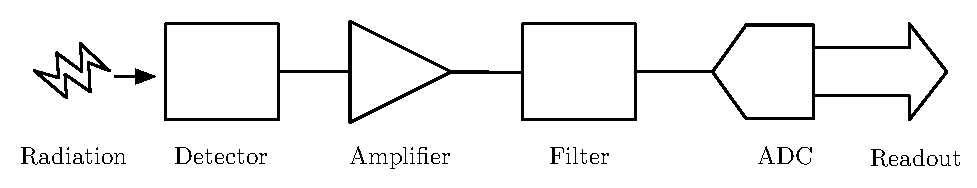
\includegraphics[width=5in]{./Figures/detector.eps}
	\caption{Block diagram for a single channel, generic instrumentation circuit for particle physics experiments.}
	\label{fig:intint}
\end{figure}

The initial amplifier translates the input charge signal, coming from the detector electrodes, into an output voltage signal. Charge-to-voltage translation is done by transferring the charge $Q_{in}$ from the nonlinear detector capacitance to a linear, known capacitor $C$. The generated voltage $V_{out}$ is simply given by $V_{out} = Q_{in}/C$, with $C$ easily and precisely tailorable. Fig.~\ref{fig:csa_post} depict the most common preamplifier implementation, which consists of a voltage amplifier with a capacitor in negative feedback configuration. The resulting feedback circuit is a charge-sensitive amplifier (CSA), extensively studied in the literature \citep{Snoeys100,Asp100,deGeronimo500,oconnor100,Alvarez101}. The amplified detector signal includes noise from the detector and the amplifier. Since the noise statistics are well modeled, they can be used to design a filter that maximizes the signal-to-noise ratio (SNR) at the detector front-end. Usually the filter is an analog block, either time-invariant or time-varying, used to convert the voltage signal at the CSA output into a shaped voltage pulse. The pulse shape defines the weights of white series, white parallel and flicker series noise sources on the front-end output noise, thus a proper selection of the pulse shape form part of the solution to the SNR maximization problem. A memory acts as a buffer necessary to store data for a number of events before readout. For high-frequency pulse trains, analog memory is particularly well suited \citep{Kleinfelder100,Haller100}. Filtered signals can be quickly stored as charge in integrated capacitors, to be converted into digital signals by dedicated ADCs during the readout phase. Integration and feature size reduction has allowed the design of highly dense digital memory arrays. If a digital memory is used instead, ADCs are used to digitize the signal prior to storage, and conversion throughput per IC must be as high as the collision rate times the number of channels. 

\begin{figure}[!t]
	\centering
	\includegraphics[width=2in]{./Figures/csa_post}
	\caption{CSA using a voltage amplifier. Detector is modeled as a photodiode.}\label{fig:csa_post}
\end{figure}


\section{Noise minimization in circuits for particle physics instrumentation}

Noise minimization in particle physics experiments is done by a careful design of the channel, and specifically, on the detector, CSA and filter parameters. Understanding and designing for low noise has been one of the main concerns in modern particle physics instrumentation. Any survey on this topic starts with a work published in 1968 \citep{radeka104}, where important concepts of pulse shaping for particle physics experiments were described. At this time, the search of practical optimum shapers and simpler analysis methods were the main concerns. The concept of a weighting function, equivalent to impulse response, but valid for time-varying systems as well, was introduced.

In 1972, a powerful time-domain analysis technique was published \citep{goulding101}, for comparing the filtering effects of different pulse shapers. Starting from a physical approach and assuming only white noise, it was shown that all the noise sources in a front-end for particle physics experiments can be reduced to two components at the input node: step (parallel) noise and delta (series) noise. Integration of each component in frequency yields two noise coefficients that make it possible to characterize the noise-filtering capabilities of a pulse shaper, independently of the time scale. These ideas are still in use today.

In 1984, a good review and some examples of readout electronics techniques for semiconductor detectors in particle physics instrumentation systems was published \citep{gatti103}. The author emphasized the importance of the input stage of the front-end electronics in the overall noise performance. By that time, there was already some interest in MOS technology (with lower performance than JFETs or MESFETs) due to the potential of integrating the semiconductor detector and its electronics. In the same year, a good summary of semiconductor position-sensitive detectors was also published \citep{radeka105}. It was shown that the minimum noise is achieved when the detector and amplifier input capacitances are matched.

In 1988, one of the most influential papers in low-noise techniques for particle physics instrumentation was published \citep{radeka101}. In this paper, the results from previous works on noise were summarized.

Flicker noise research in particle physics electronics was published in 1989 \citep{lutz101}. Before this paper, flicker noise was rarely mentioned and seldom considered in analysis equations for particle physics electronics. In 1990, the issue of optimum shapers for particle physics electronics, including low frequency noise in the analysis, was published \citep{gatti104}. The same year, an excellent derivation of noise for particle physics front-end electronics, including thermal, flicker and shot noise sources was presented \citep{sansen101}.

In 1992 \citep{gadomski101}, the deconvolution method for pulse-shaping was presented. Major innovations of this work come from the use of switched-capacitor filters for \mbox{pulse-processing} purposes and the introduction of the concept of \mbox{discrete-time} \mbox{pulse-shaping}.

In 1998 \citep{pullia104}, for the first time the contribution of the low-frequency noise is computed in the time domain, using fractional derivatives. It is an extension of earlier noise computation methods \citep{goulding101}. A generalization of this work was presented in 2004 \citep{pullia102}, allowing time-domain simulations of almost all kind of noise sources.  A powerful tool for computer-aided filter design.


%In 2001, a nice overview of front-end electronics for imaging detectors, oriented to particle physics applications was published [7]. In that work, neat and simple equations to compute the equivalent noise charge from white, flicker and shot sources were presented. The same equations are employed in a later publication [12], where it is shown that, using more accurate transistor and noise models, minimum noise is not necessarily achieved when maximum available power and capacitance matching conditions are fulfilled. 
%It is also shown that the low frequency noise contribution may depend on the shaper time constant, a result not found before using simpler equations.

Finally, excellent books on particle physics instrumentation systems have been published \citep{radeka201}, compiling and explaining the results from many papers in the field.


\section{Thesis content}
Chapter 2 starts with an introduction to the project that prompt the work of this thesis, the design and implementation of a second iteration of The Bean, an instrumentation application-specific integrated circuit (ASIC) which forms part of the proposal for the ILC. It is followed by an overview of the motivations that lead to the development of a new mathematical framework for noise analysis in discrete-time filters, alongside with the presentation of the requirements for a filter intended to take full advantage of this framework. Chapter 3 presents the complete formulation of this noise analysis, including examples and applications for optimal filter computation. In Chapter 4 , the design and implementation of a filter for arbitrary weighting function synthesis are presented. Chapter 5 shows the results that contribute to the ongoing project, functionality verifications of the designed filter and the implementation of an early prototype of The Bean 2, with the filter as one of its core building blocks. Finally, Chapter 6 summarizes the results and contributions of this work, and presents ideas for future research.
\clearpage
\chapter{PROBLEM DEFINITION}
\label{chapter:problem}
\section{The International Linear Collider}

The work described in this thesis form part of the design and implementation of the front-end circuit for one of the detector systems of the International Linear Collider (ILC).

Planned to be operating in the mid 2020’s, the ILC will be the largest linear collider ever built. Consisting of two linear accelerators that will stretch approximately 32 kilometers in length, the ILC will smash electrons and positrons together at nearly the speed of light. The intended beam collision energy is 500 billion-electron-volts (GeV) for the first stage, with the possibility for a later upgrade to 1 TeV. 




Superconducting accelerator cavities operating at temperatures near absolute zero give the particles more and more energy until they smash in centre of the machine, where a bunch of detectors gather clues about the particles identity .
 
Located at the ILC detector forward region, the BeamCal is a highly segmented ($>$ 90000 channels) calorimeter that will serve three main purposes: improve the hermeticity of the ILC detector for low polar angles, reduce the backscattering from pairs into the inner ILC detector part and protect the final magnet of the beam delivery system, and assist the beam diagnostics. The BeamCal specifications for radiation tolerance, noise, signal charge, pulse rate and occupancy pose unique challenges for the instrumentation system.

The project FONDECYT 11110165: Application of Advanced CMOS Techniques in Pulse Processors for Particle Physics Experiments deals with the design and implementation of a mixed-signal integrated circuit (IC) to address the BeamCal instrumentation needs.

\section{The Bean}
The Bean – BeamCal Instrumentation IC – is a 32-channel front-end and readout ASIC that will address the BeamCal instrumentation requirements. By employing a charge-sensitive amplifier and a switched-capacitor filter, the Bean will process the input charge signals at the ILC pulse rate. Each channel will have a 10-bit successive approximation register analog-to-digital converter and digital memory for readout purposes. The Bean will also feature a fast feedback adder, capable of providing an 8-bit, low-latency output for beam diagnostics purposes.

\begin{table}[!t]
	\begin{center}
		\begin{tabular}{|l|l|}\hline
			Input rate & $3.25\,\text{MHz}$ during $0.87\,\text{ms}$, repeated every $200\,\text{ms}$ \\ \hline
			Channels per ASIC & $32$ \\ \hline
			Occupancy & $100\%$ \\ \hline
			Resolution & 10 bits for individual channels, 8 bits for fast feedback \\ \hline
			Modes of operation & Standard data taking (SDT), Detector Calibration (DCal) \\ \hline
			Input signals & 4 fC - 40 pC in SDT, 0.74 pC in DCal \\ \hline
			Input capacitance & 65 pF \\ \hline
			Additional feature & Low-latency ($1\,\micro\text{s}$) output \\ \hline
			Additional feature & Internal pulser for electronics calibration \\ \hline
			Radiation tolerance & 1 Mrad ($\text{SiO}_2$) total ionizing dose \\ \hline
			Power consumption & 2.19 mW per channel \\ \hline
			Total ASIC count & $2836$ \\\hline
		\end{tabular}
		\vspace*{5pt}
		\caption{BeamCal instrumentation ASIC specifications summary.}\label{tab:bean_specs}
	\end{center}
\end{table}

\begin{table}[!t]
	\begin{center}
		\begin{tabular}{|l|l|}\hline
			{\bf Noise source} & {\bf Noise power budget} \\ \hline\hline
			CSA & $1\times Q_n^2$ \\ \hline
			Filter $kT/C$ & $1\times Q_n^2$ \\ \hline
			Filter amplifier & $0.25\times Q_n^2$ \\\hline 
			Buffers & $0.25\times Q_n^2$ \\ \hline
			ADC & $0.25\times Q_n^2$ \\ \hline
			Total & $2.75\times Q_n^2$ \\\hline
		\end{tabular}
		\vspace*{5pt}
		\caption{Channel noise budget.}\label{tab:noise_budget}
	\end{center}
\end{table}
\clearpage
\chapter{NOISE ANALYSIS IN PULSE-PROCESSING DISCRETE-TIME FILTERS\footnotemark}
\label{chapter:theoretical}
\section{Introduction}
\footnotetext{See also \citep{avila101}}
In particle physics experiments, where the results from the collisions are inferred from the measurement of electric charge in various sets of detectors \citep{gatti101,radeka101}, noise sets a fundamental limit for the charge measurement resolution \citep{degeronimo102}. In such experiments, the typical detector \mbox{front-end} circuit comprises a \mbox{charge-sensitive} amplifier (CSA) and a filter, often referred to as pulse shaper. The former is used to convert the input charge signal, coming from the detector electrodes, into a voltage signal, and is responsible for most of the noise present in the readout circuit signal path \citep{degeronimo101,degeronimo102}. The filter is used to convert the voltage signal at the CSA output into a shaped voltage pulse, in order to maximize the \mbox{signal-to-noise} ratio (SNR) at the measurement time.

Different noise analysis methods have been proposed to guide a proper filter design. The outcome of these methods is the equivalent noise charge ($\mathit{ENC}$), a measure of the \mbox{front-end} noise defined as the charge required at the detector input to produce an output SNR  of $1$. A \mbox{time-domain} analysis based on the weighting function (WF) concept \citep{radeka101, goulding101} has long been the preferred analysis, since it allows to find the optimum filter for a wide range of detector configurations \citep{radeka104,geraci101, gatti102,pullia103,pullia105}.

Traditionally, the filter synthesis has been performed using \mbox{continuous-time} networks. However, since producing arbitrary WFs by means of \mbox{continuous-time} analog circuitry is often impossible \citep{gatti102}, this approach does not always allow to synthesize optimum filters. A different approach based on \mbox{discrete-time} filters, implemented by means of digital signal processor (DSP) units \citep{geraci103,sampietro101,jordanov101} or switched capacitor networks \citep{porro101,fiorini101,abusleme101}, allows to synthesize WFs with virtually any shape, producing \mbox{near-optimum} filters. Moreover, this promising approach takes advantage of the aggressive technology scaling and the new techniques of the VLSI industry, allowing to implement fast, reliable and flexible filters.

In this work, a mathematical framework for a \mbox{design-oriented} analysis of \mbox{discrete-time} filters in the \mbox{discrete-time} domain is presented. Although \mbox{discrete-time} filters can be analyzed using a \mbox{continuous-time} method, it is not insightful and the resulting expressions are complex and difficult to use for design purposes. Furthermore, the analysis of \mbox{discrete-time} filters in the \mbox{discrete-time} domain provides a better insight on how their discrete nature affects the \mbox{front-end} noise. The proposed analysis can produce \mbox{closed-form} expressions for the $\mathit{ENC}$ calculation, which can be used for efficient algorithms for the $\mathit{ENC}$ evaluation and filter optimization procedures.

In order to validate the proposed framework in this work, an example is developed, and the result obtained is analyzed and compared with the result provided by the \mbox{continuous-time} approach. Also, an example of optimal filter computation is presented to demonstrate the capabilities of the proposed framework.


%%%%%%%%%%%%%%%%%%%%%%%%%%%%%%%%%%%%%%%%%%%%%%%%%%%%%%%%%%%%%%%%%%%%%%%%%%%%%%
%%%%%%%%%%% SECTION II: DISCRETE-TIME ANALYSIS %%%%%%%%%%%%%%%%%%%%%%%%%%%%%%%
%%%%%%%%%%%%%%%%%%%%%%%%%%%%%%%%%%%%%%%%%%%%%%%%%%%%%%%%%%%%%%%%%%%%%%%%%%%%%%
\section{Discrete-Time Analysis}

\figurename~\ref{fig:system} shows a simplified model to compute the \mbox{output-referred} noise contribution of a single noise source in a typical \mbox{front-end} detector. It consists of a linear block with a transfer function $H(s)$ that models the effect of the CSA on the noise source under analysis, and a \mbox{pulse shaper}, which in this case is a finite impulse response (FIR) filter with a \mbox{discrete-time} transfer function given by
\begin{equation}
F(z) = \sum_{j=0}^{N-1}a_{N-j} \hspace{0.1em}z^{-j} \label{eq:FIRtf}
\end{equation}
where $a_{N-j}$ are arbitrary coefficients and $N$ is the filter length. The noise source is characterized by its \mbox{two-sided} power spectral density (PSD) $\overline{n^2}(f)$.

For this analysis it is not necessary to consider the details of the physical processes that cause the noise. It will be assumed that the noise source is an arbitrary white or filtered white noise source, which represents any of the fundamental noise sources present at a detector front-end circuit, such as thermal noise, shot noise and flicker noise. This assumption allows to model the noise source in the time domain in terms of a sequence of noise pulses with core function $y(t)$, arriving Poissonianly at times $t_a$ with an average rate $\nu$ and random sign \citep{radeka101, goulding101}. A general procedure to calculate a function $y(t)$ that represents the noise process characterized by $\overline{n^2}(f)$ can be found in \citep{pullia102}.

By using the CSA transfer function and $y(t)$, the effect of an individual noise pulse at the filter input can be determined as
\begin{equation}
\hat{y}(t) = y(t) \ast \mathcal{L}^{-1}\!\left\{ H(s)\right\}\hspace{-0.15em}(t).\label{eq:shaped-pulse}
\end{equation}
Both sequences of pulses, at the input and at the output of $H(s)$, are illustrated in \figurename~\ref{fig:system}.

\begin{figure}[!t]
	\centering
	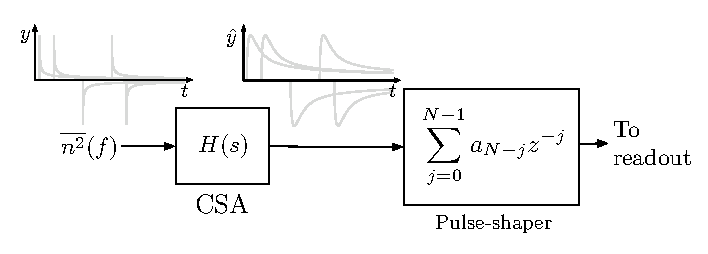
\includegraphics[width=4in]{./Figures/system.eps}
	\caption{Model for noise analysis in a typical \mbox{front-end} circuit.}\label{fig:system}
\end{figure}

Assuming a periodic, synchronous \mbox{front-end}, where the stimulus arrival time within each frame is fixed and known, the CSA can be reset at the beginning of each frame, prior to the corresponding stimulus. Thus, the analysis can be carried out considering a non-stationary noise process that starts at $t=0$. Then the total integrated noise at the filter input is a function of time \citep{radeka201}. Using \eqref{eq:shaped-pulse} and Campbell's theorem, the following expression for the total integrated noise at the filter input can be derived:
\begin{equation}
\sigma^2(t) = \nu\hspace{-.25em}\int_{0}^{t}\hspace{-.45em}\hat {y}^2(t-t_a)\;\mathrm{d}t_a\label{eq:envelope}.
\end{equation}

Let us define $P_i$ as the time interval between an arbitrary sample $i$ and its predecessor, given by $P_i=[(i-1)T_s, iT_s]$, where $T_s$ is the filter sampling period. Now consider the noise contribution of the pulses originated within $P_i$ and measured at an arbitrary sample $k$ (i.e., $t=kT_s$), $\sigma_i^2(k)$, as shown in \figurename~\ref{fig:sequence}. Using Campbell's theorem,  $\sigma_i^2(k)$ can be computed as
\begin{equation}
\sigma_i^2(k) = \nu\hspace{-.25em} \int_{(i-1)T_s}^{iT_s} \hspace{-.15em}  \hat{y}^2(kT_s-t_a)\;\mathrm{d}t_a\hspace{0.1em}. \label{eq:int2}
\end{equation}
It can be shown that \eqref{eq:int2}, can be expressed as
\begin{equation}
		\sigma_i^2(k) = \int_{0}^{T_s} \hspace{-.45em} \hat{y}^2\left(\left(k-i+1\right)T_s-\eta_1\right)\; \mathrm{d}\eta_1 
		\label{eq:ap1}
\end{equation}
where $\eta_1 = t_a+T_s-iT_s$. This integral can be split into two integrals as follows
\begin{eqnarray}
		\sigma_i^2(k) \hspace{-0.6em} &=& \hspace{-0.6em} \int_{0}^{(k-i+1)T_s} \hspace{-.65em} \hat{y}^2\left(\left(k-i+1\right)T_s-\eta_1\right)\; \mathrm{d}\eta_1 \nonumber\\
		&&\hspace{-0.8em}{-}\: \int_{T_s}^{(k-i+1)T_s} \hspace{-.65em} \hat{y}^2\left(\left(k-i+1\right)T_s-\eta_2\right)\; \mathrm{d}\eta_2.  
		\label{eq:ap2}
\end{eqnarray}
Defining $\eta_2 = \eta_3 + T_s$,~\eqref{eq:ap2} can be written as
\begin{eqnarray}
		\sigma_i^2(k) &=& \int_{0}^{(k-i+1)T_s} \hspace{-.45em} \hat{y}^2\left(\left(k-i+1\right)T_s-\eta_1\right)\; \mathrm{d}\eta_1 \nonumber\\
		&&{-}\: \int_{0}^{(k-i)T_s} \hspace{-.45em} \hat{y}^2\left(\left(k-i\right)T_s-\eta_3\right)\; \mathrm{d}\eta_3.  
		\label{eq:ap3}
\end{eqnarray}
Since $\hat{y}^2(t)$ is zero for negative arguments, then \mbox{$\sigma_i^2(k)= 0$} for $k < i$. For $k \geq i$, and according to~\eqref{eq:envelope},~\eqref{eq:ap3} can be alternatively expressed as
\begin{equation}
		\sigma_i^2(k) = \sigma^2\left(\left(k-i+1\right)T_s\right)-\sigma^2\left(\left(k-i\right)T_s\right) 
		\label{eq:ap4}
\end{equation}
therefore,
\begin{equation}
  \sigma_i^2(k) \hspace{-0.2em}=\hspace{-0.2em} 
  \begin{cases}
     \sigma^2((k-i+1)T_s)-\sigma^2((k-i)T_s ), & k \geq i   \\
      0, &   k < i.
  \end{cases}\label{eq:sigmaj}
\end{equation}

\begin{figure}[!t]
	\centering
	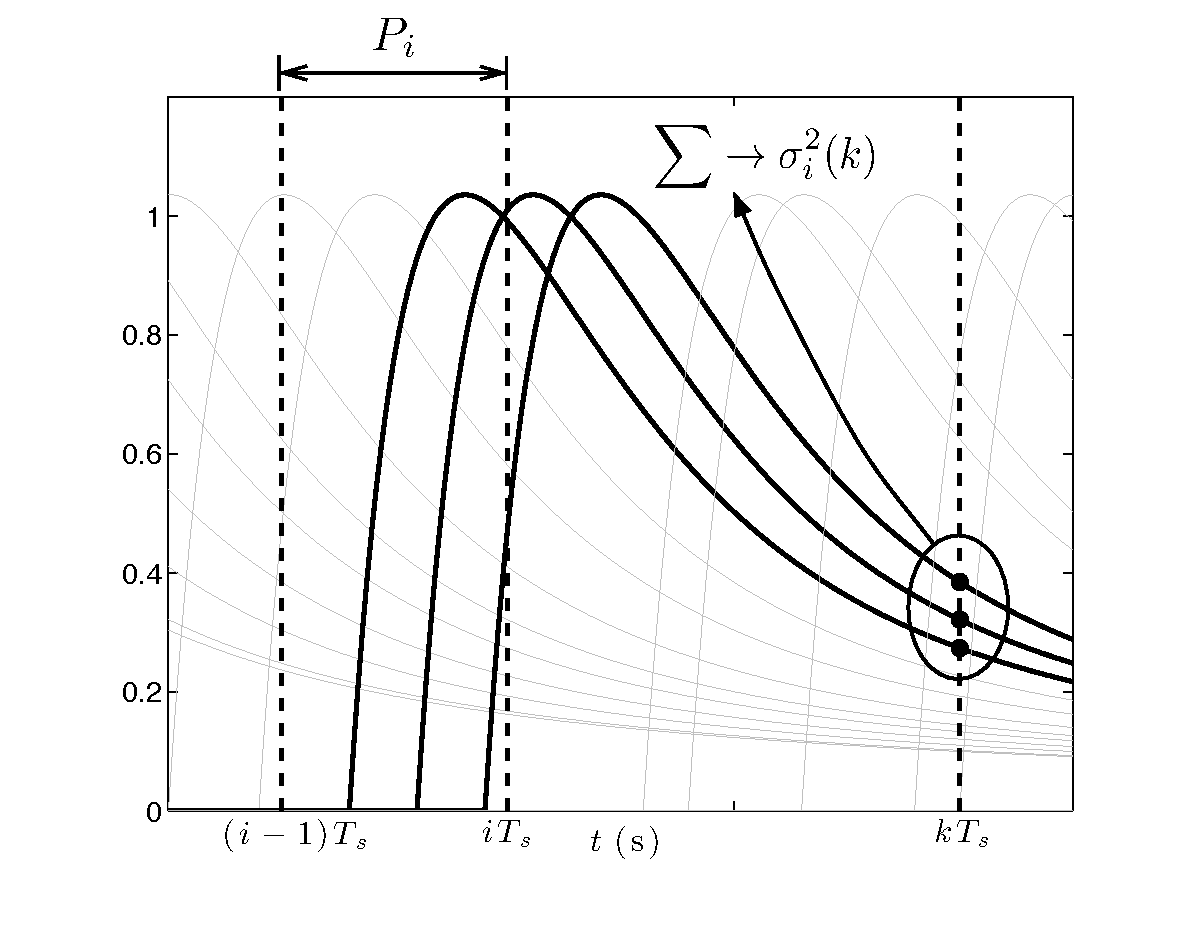
\includegraphics[width=4.5in]{./Figures/sequence.eps}
	\caption{Noise contribution of the pulses generated within $P_i$ and measured at an arbitrary sample $k$ (i.e., $t=kT_s$), using an arbitrary filtered noise core function $\hat{y}(t)$. The independent contribution of each pulse is pointed out with black dots.}\label{fig:sequence}
\end{figure}

Based on \eqref{eq:sigmaj}, the total integrated noise at the filter input measured at the \mbox{$k$-th} sample, $\sigma^2(kT_s)$, can be written as the sum of the individual noise contributions originated at each interval $P_i$:
\begin{equation}
\sigma^2(kT_s) = \sum_{i=1}^{N} \sigma_i^2(k). \label{eq:noise_evo}
\end{equation}
The evolution of the total integrated noise at the filter input according to \eqref{eq:noise_evo} is illustrated in \figurename~\ref{fig:envelope-example}. 

Since \eqref{eq:noise_evo} is composed by noise contributions originated at different time intervals $P_i$, the total integrated noise at the filter input holds partial correlation between samples, and the output noise cannot be computed by convolving \eqref{eq:noise_evo} with $F(z)$. However, since all evaluations of $\sigma_i^2(k)$ are originated from the same pulses (for a fixed $i$), and thus are fully correlated, \eqref{eq:noise_evo} can be split into $N$ independent \mbox{discrete-time} signals $\sigma_1^2(k), \sigma_2^2(k) \ldots \sigma_N^2(k)$. Each of these signals can be referred to the filter output as
\begin{align}
\hat{\sigma}_i(k) &= \sqrt{\sigma^2_i(k) } \ast \mathcal{Z}^{-1}\!\left\{ F(z) \right\}\hspace{-0.15em}(k) \nonumber \\
          &= \sum_{j=0}^{k-i} a_{N-j} \sqrt{\sigma^2_i(k-j)}.  \label{eq:sigmao}
\end{align}
Signals $\hat{\sigma}_1(k), \hat{\sigma}_2(k) \ldots \hat{\sigma}_N(k)$ are also independent, and can be added up as noise variances to compute the total integrated noise at the filter output as a function of $k$:
\begin{align}
\hat{\sigma}^2(k) &= \sum_{i=1}^k \hat{\sigma}_i^2(k) \nonumber \\
		       &= \sum_{i=1}^k \left(\sum_{j=0}^{k-i} a_{N-j}\sqrt{\sigma_i^2(k-j)}\right)^2 \hspace*{-7pt}.  \label{eq:sigmatk}
\end{align}
Evaluating \eqref{eq:sigmatk} at the measurement time \mbox{$t_m=NT_s$} \mbox{(i.e., $k=N$)} yields
\begin{align}
\hat{\sigma}^2(N) = \sum_{i=1}^N \left(\sum_{j=0}^{N-i} a_{N-j}\sqrt{\sigma_i^2(N-j)}\right)^2\hspace*{-7pt}.\hspace{0.2em} \label{eq:sigmaNprev}
\end{align}
Finally, replacing \eqref{eq:sigmaj} in \eqref{eq:sigmaNprev} and defining $h = N-j-i$, a closed-form expression for the front-end noise can be obtained:
\begin{equation}
\hat{\sigma}^2(N) = \sum_{i=1}^N \left( \sum_{h=0}^{N-i} a_{i+h} \sqrt{\sigma^2((h+1)T_s)-\sigma^2(hT_s)}\right)^2\hspace{-0.5em}. \label{eq:final}
\end{equation}

\begin{figure}[!t]
	\centering
	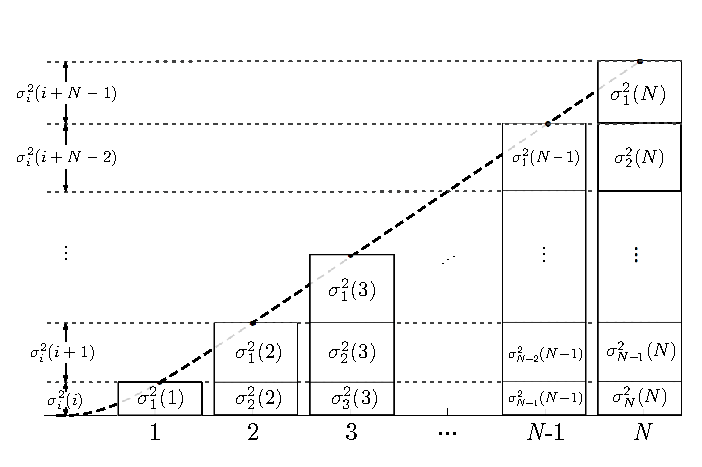
\includegraphics[width=5in]{./Figures/envelope-example.eps}
	\caption{Evolution of the total integrated noise at the filter input, where the noise of each sample was split according to \eqref{eq:noise_evo}.}\label{fig:envelope-example}
\end{figure}

The only term of \eqref{eq:final} that depends on the input-referred noise process is $\sigma^2(t)$, which can be calculated analytically or numerically for typical noise processes by using \eqref{eq:envelope}. For instance, \figurename~\ref{fig:envelopes} illustrates $\sigma^2(t)$ for thermal, shot and flicker noise. Even though the analysis presented here has been applied for a single noise source, it can be easily extended for circuits with several noise sources by applying the superposition principle in quadrature. 

\begin{figure}[!t]
	\centering
	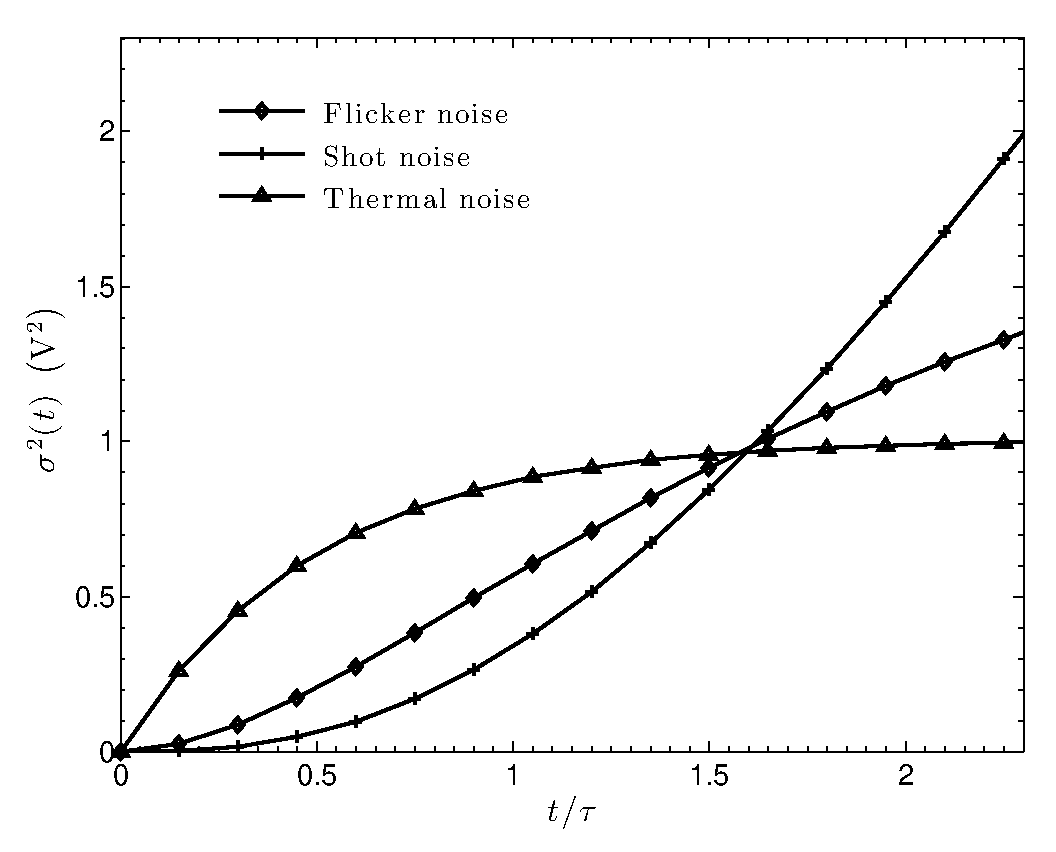
\includegraphics[width=4.2in]{./Figures/envelopes.eps}
	\caption{$\sigma^2(t)$ for thermal, shot and flicker noise with normalized time $t/\tau$ and an arbitrary amplitude.}\label{fig:envelopes}
\end{figure}

%%%%%%%%%%%%%%%%%%%%%%%%%%%%%%%%%%%%%%%%%%%%%%%%%%%%%%%%%%%%%%%%%%%%%%%%%%%%%%
%%%%%%%%%%% SECTION III: EXAMPLE %%%%%%%%%%%%%%%%%%%%%%%%%%%%%%%%%%%%%%%%%%%%%
%%%%%%%%%%%%%%%%%%%%%%%%%%%%%%%%%%%%%%%%%%%%%%%%%%%%%%%%%%%%%%%%%%%%%%%%%%%%%%
\section{Example}
For validation purposes, the thermal noise contribution at the output of a \mbox{discrete-time} integrator filter will be computed using the proposed \mbox{discrete-time} analysis. The result obtained will be analyzed and then compared with the result produced by the traditional \mbox{continuous-time} approach. \figurename~\ref{fig:analysis-circuit} shows the front-end circuit used for general noise analysis. The detector is modeled as capacitance $C_D$, whereas the CSA is shown as a voltage amplifier with open loop gain $A(s) = A/(1+s\tau)$, input capacitance $C_{in}$ and a feedback capacitor $C_F$. Resistor $R_R$ across the feedback capacitor $C_F$ represents the CSA reset element. The filter coefficients are $a_i=1$. The detector shot noise represented by $\overline{i^2_D}$ will be omitted for the purpose of this example. Thermal noise has been assumed to be dominated by the CSA input device and is represented by two \mbox{fully-correlated} noise sources \citep{sansen101}, a voltage white noise source with a \mbox{two-sided} PSD $\overline{v_n^2}$ and a current noise source with a \mbox{two-sided} PSD $\overline{i_n^2}$. Both noise sources are related as follows:
\begin{equation} 
\overline{i_n^2} = (sC_{in})^2 \hspace{0.2em}\overline{v_n^2}\label{eq:current}.
\end{equation}

Considering that the effect of the reset switch during the relatively short time that it takes the CSA to produce an output voltage is negligible, $R_R$ can be assumed to be infinite \citep{pullia102}. The CSA open loop DC gain ($A$) is assumed to be very large as well. Under these assumptions and using \eqref{eq:current}, the PSD of the thermal noise referred to the CSA output, $\overline{v_o^2}$, can be approximated to
\begin{equation} 
	\overline{v_o^2} \approx \left|\frac{C_{tot}}{C_f} \frac{1}{1+s\hat{\tau}}\right|^2\overline{v_n^2} \label{eq:ex-PSD}
\end{equation}
where $C_{tot} = C_D+C_F+C_{in}$ and $\hat{\tau} = (\tau/A) (\hspace{0.2em}C_{tot}/C_f)$ is the CSA \mbox{closed-loop} \mbox{time-constant}.

\begin{figure}[!t]
	\centering
	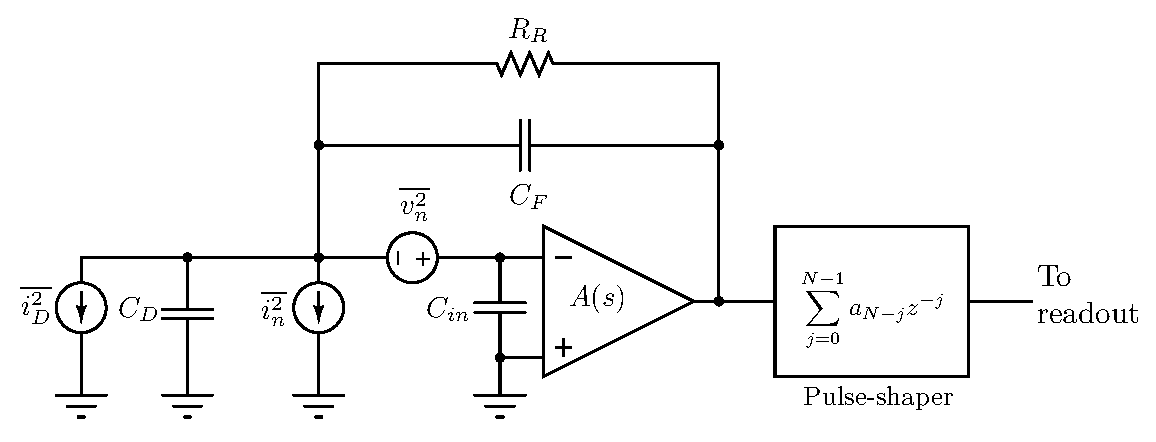
\includegraphics[width=5in]{./Figures/front-end.eps}
	\caption{Front-end circuit used for noise analysis.}\label{fig:analysis-circuit}
\end{figure}

The PSD in \eqref{eq:ex-PSD} can be treated as the result of passing a fictitious noise source with PSD $\overline{v_n^2}$ through a block with transfer function $H_\text{th}(s)$ given by
	\begin{equation} 
		H_\text{th}(s) =  \frac{C_{tot}}{C_f}\frac{1}{1+s\hat{\tau}}. \label{eq:exampletf}
	\end{equation}

Since $\overline{v_n^2}$ characterizes a white noise source, it can be modeled as a sequence of Dirac impulses with core function $y_\text{th}(t)$ occurring at an arbitrary rate $\nu$ and random sign \citep{pullia102}, where $y_\text{th}(t)$ is given by
	\begin{equation} 
		y_\text{th}(t) = \sqrt{\frac{\overline{v_n^2}}{\nu}}\delta(t)\label{eq:pulseW}.
	\end{equation}
Replacing \eqref{eq:exampletf} and \eqref{eq:pulseW} in \eqref{eq:shaped-pulse}, each pulse in the sequence can be referred to the CSA output as an exponentially decaying pulse \citep{pullia102} as follows
	\begin{equation} 
		\hat{y}_\text{th}(t-t_a)  = \sqrt{\frac{\overline{v_n^2}}{\nu}}\frac{C_{tot}}{C_F} \frac{ e^{-(t-t_a)/\hat{\tau}}}{\hat{\tau}}u(t-t_{a}) \label{eq:shapedW}
	\end{equation}
where $u(t)$ is the unit step function. Substituting \eqref{eq:shapedW} in \eqref{eq:envelope}, the filter input total integrated noise due to the thermal noise, $\sigma_\text{th}^2(t)$, can be derived:
	\begin{equation} 
		\sigma_\text{th}^2(t) = \overline{v_n^2} \frac{C_{tot}^2}{C_F^2}  \frac{1-e^{-2t/\hat{\tau}}}{2\hat{\tau}}u(t). \label{eq:envelopeW}
	\end{equation}
Finally, replacing \eqref{eq:envelopeW} in \eqref{eq:final} and defining $x=e^{T_s/\hat{\tau}}$, the front-end noise, $\hat{\sigma}_\text{th}^2(N)$, can be obtained:
	\begin{equation}
	\hat{\sigma}_\text{th}^2(N)  = \frac{\overline{v_n^2}}{2\hat{\tau}}\frac{C_{tot}^2}{C_F^2}\frac{\left(N(x^2\hspace{-0.1em}-\hspace{-0.1em}1) \hspace{-0.1em}-		\hspace{-0.1em}2x\hspace{-0.1em}-\hspace{-0.1em}x^{-{2N}}\hspace{-0.25em}+\hspace{-0.1em}2x^{-{N}}\hspace{-0.25em}+\hspace{-0.1em}2x^{1-N}		\hspace{-0.2em}-1 \right)}{(x-1)^2}\hspace{-2pt}.   \label{eq:exFinal}
	\end{equation}
	
When the time interval between samples is large enough to consider that consecutive noise samples are uncorrelated \mbox{(i.e., $\hat{\tau} \ll T_s$),} $\hat{\sigma}_\text{th}^2(N)$ can be approximated without the use of the proposed analysis as a weighted sum of the uncorrelated samples of the total integrated noise at the CSA output as follows:
\begin{equation}
	\left. \hat{\sigma}_\text{th}^2(N)\right\rvert_{\hat{\tau}\ll T_s}  \approx  N \lim_{t\rightarrow \infty} \sigma^2(t) = N \frac{\overline{v_n^2}}{2\hat{\tau}}\frac{C_{tot}^2}{C_F^2}. \label{eq:aprox}
\end{equation}

As shown in \figurename~\ref{fig:exampleSigma}, \eqref{eq:exFinal} behaves as predicted by \eqref{eq:aprox} for small values of $\hat{\tau}$.
\begin{figure}[!t]
	\centering
	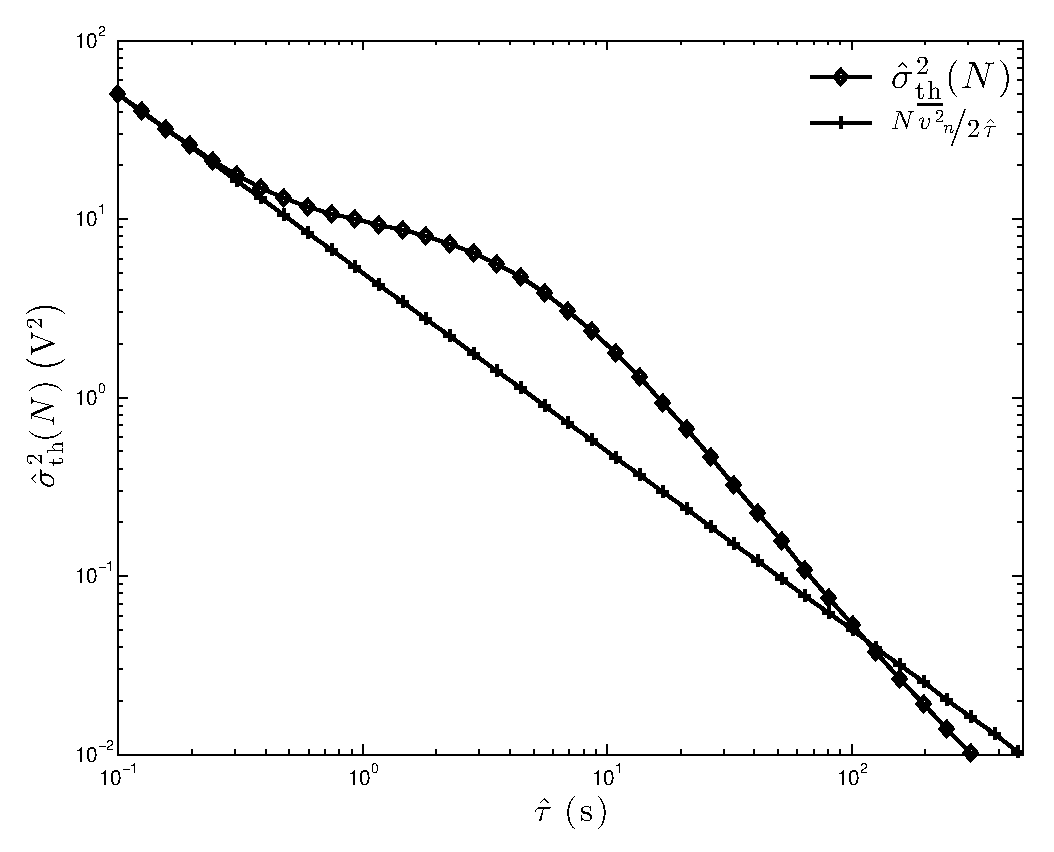
\includegraphics[width=4in]{./Figures/example.eps}
	\caption{$\hat{\sigma}_\text{th}^2(N)$  and $N \frac{\overline{v_n^2}}{2\hat{\tau}}\frac{C_{tot}^2}{C_F^2}$ as a function of $\hat{\tau}$, using $\overline{v_n^2} = 1$, \mbox{$C_{tot}^2/C_F^2 = 1$} and $N = 20$.}\label{fig:exampleSigma}
\end{figure}

Now, the same example will be analyzed using the traditional \mbox{continuous-time} approach. Using \eqref{eq:shapedW}, the WF $w(t)$, defined as the contribution of each pulse occurring at time $t$ measured at a fixed time $t_m=NT_s$ at the output of the filter, is given by
\begin{align}
	w(t) &= \sum_{n=1}^{N} \hat{y}_\text{th}(nT_s-t) \nonumber \\
       	 &=\sqrt{\frac{\overline{v_n^2}}{\nu}} \frac{C_{tot}}{C_F}\sum_{n=1}^{N} \frac{e^{-(nT_s-t)/\hat{\tau}}}{\hat{\tau}} u(nT_s-t) \label{eq:WF}.
\end{align}
Integrating \eqref{eq:WF} from the reset time ($t=0$) to the signal measurement time ($t=t_m$), the filter total integrated noise at $t=t_m$ can be computed as
\begin{align} 
	\hat{\sigma}_\text{th}^2(N) &= \nu \hspace{-0.3em}\int_{0}^{t_m}\hspace{-0.5em}w^2(t)\,\text{d}t \nonumber \\
									&= \overline{v_n^2} \frac{C_{tot}^2}{C_F^2} \int_{0}^{NT_s} \hspace{-0.4em}\left(\sum_{n=1}^{N} \frac{e^{-(nT_s-t)/\hat{\tau}}}{\hat{\tau}} u(nT_s-t)\right)^{\hspace{-0.2em}2}\hspace{-0.4em}\text{d}t \label{eq:pre1}.
\end{align}
Defining $\alpha = T_s/\hat{\tau}$ and $\beta = t/\hat{\tau}$, \eqref{eq:pre1} can be \mbox{re-written} as
\begin{equation}
	\hat{\sigma}_\text{th}^2(N)   = \frac{\overline{v_n^2}}{\hat{\tau}}\frac{C_{tot}^2}{C_F^2}\int_{0}^{N\alpha}e^{2\beta} \left(\sum_{n=1}^{N}e^{-n\alpha}u\left(n\alpha-\beta\right) \right)^{\hspace{-0.3em}2}\hspace{-0.1em}\text{d}\beta \label{eq:pre2}
\end{equation}
which can be split into a sum of integrals as follows
\begin{equation}
	\hat{\sigma}_\text{th}^2(N) = \frac{\overline{v_n^2}}{\hat{\tau}}\frac{C_{tot}^2}{C_F^2}\sum_{n=1}^{N}\int_{(n-1)\alpha}^{n \alpha} e^{2\beta} \left(\sum_{k = n}^{N} e^{-k\alpha}\right)^{\hspace{-0.3em}2}\hspace{-0.1em}\text{d}\beta \label{eq:pre3}.
\end{equation}
Finally, defining $x= e^{\alpha}$ it can be shown that \eqref{eq:pre3} is equal to \eqref{eq:exFinal}.

%%%%%%%%%%%%%%%%%%%%%%%%%%%%%%%%%%%%%%%%%%%%%%%%%%%%%%%%%%%%%%%%%%%%%%%%%%%%%%
%%%%%%%%%%% SECTION IV: OPTIMIZATION %%%%%%%%%%%%%%%%%%%%%%%%%%%%%%%%%%%%%%%%%
%%%%%%%%%%%%%%%%%%%%%%%%%%%%%%%%%%%%%%%%%%%%%%%%%%%%%%%%%%%%%%%%%%%%%%%%%%%%%%
\section{$\mathit{ENC}$ Minimization}

For filter optimization purposes, a typical \mbox{front-end} circuit with thermal, shot and flicker noise components is considered. The \mbox{front-end} configuration from \figurename~\ref{fig:analysis-circuit} will be used. In this case, the pulse shaper is a \mbox{discrete-time} FIR filter with indeterminate coefficients $a_i$. Shot noise is assumed to be dominated by the detector noise and is represented by a white noise current source with \mbox{two-sided} PSD $\overline{i^2_D}$ in parallel with the detector capacitance $C_D$ and given by
	\begin{equation} 
		\overline{i^2_D} = qI_L
	\end{equation}
where $q$ is the electron charge and $I_L$ the detector leakage current. Thermal noise and flicker noise are assumed to be dominated by the noise of the CSA input device and are represented by two \mbox{fully-correlated} noise sources, a voltage noise source with \mbox{two-sided} PSD $\overline{v_n^2}$ given by
	\begin{equation} 
		\overline{v_n^2} =   a_T + \frac{a_F}{|f|}
	\end{equation}
where $a_T$ and $a_F$ are the thermal and flicker coefficients, and a current noise source with \mbox{two-side} PSD $\overline{i_n^2}$ given by \eqref{eq:current}. Traditionally, the coefficients $a_T$ and $a_F$ are obtained from the CSA input device models. However, for design purposes the most accurate values shall be used, and these coefficients should be extracted from experiments \citep{bertuccio101} or precise simulations.

Considering the contribution of each noise process separately, the $\mathit{ENC}^2$ for the output measured at $t = NT_s$ can be written as 
	\begin{equation}
		\mathit{ENC}^2 = \frac{\hat{\sigma}_\text{shot}^2(N)+\hat{\sigma}_\text{th}^2(N) +  \hat{\sigma}_{1/f}^2(N)}{q^2\left| \max[w(t)]		\right|^2/C_F^2}\label{eq:enc}
	\end{equation}
where $\hat{\sigma}_\text{shot}^2(N)$ is the shot noise contribution, $\hat{\sigma}_\text{th}^2(N)$ is the thermal noise contribution, $\hat{\sigma}_{1/f}^2(N)$ is the flicker noise contribution and $w(t)$ is the weighting function at the \mbox{front-end} output given by \eqref{eq:WF}.

In order to find the coefficients $a_i$ that minimize \eqref{eq:enc}, and hence the optimal FIR filter, the signal measurement time $t_m=NT_s$ was assumed to be a constant determined by the processing time budget constraints, and the filter sampling period $T_s$ was assumed to be a constant determined by the filter maximum clock rate. Although $\hat{\tau}$ is a design variable that depends on the CSA and not on the filter, it has been included in the optimization analysis. 

Given that a common WF reaches its maximum value at \mbox{$t=t_m/2$}, and that the WF height is commonly a design constraint, the denominator of \eqref{eq:enc} was forced to be constant by fixing the WF height, $h_{w}$, through the following constraints
	\begin{align}
		\sum_{i=1}^{N/2} a_{i}\left(1-e^{ - T_s(N/2-i+1)/\hat{\tau}}\right) &= h_w \label{eq:con1}\\
		\sum_{i=1}^{N} a_{i}\left(1-e^{-T_s(N-i+1)/\hat{\tau}}\right) &= 0 \label{eq:con2}.
	\end{align}
Although these constraints appear from foreknowledge about the shape of the optimum WF, the actual computation of $w(t)$ was never required for the optimization problem formulation. For illustration purposes, the length of the filter $N$ was assumed to be an even number. Considering these constraints, minimizing the $\mathit{ENC}^2$ is equivalent to minimizing its numerator, and according to \eqref{eq:final}, the resulting objective function $f_o$ is given by
	\begin{eqnarray} 
		f_o \hspace{-0.7em}&=  \hspace{-0.7em} &\sum_{i=1}^N \left\{\left( \sum_{h=0}^{N-i} a_{i+h} \sqrt{\sigma_\text{shot}^2((h+1)T_s)-\sigma_\text{shot}^2(hT_s)}\right)^{\hspace{-0.3em}2} \right.\nonumber\\
		\hspace{-1em}&  \hspace{-1em}&+ \left( \sum_{h=0}^{N-i} a_{i+h} \sqrt{\sigma_\text{th}^2((h+1)T_s)-\sigma_\text{th}^2(hT_s)}\right)^{\hspace{-0.3em}2} \nonumber\\
		\hspace{-1em}&  \hspace{-1em}& + \left.\left( \sum_{h=0}^{N-i} a_{i+h} \sqrt{\sigma_{1/f}^2((h+1)T_s)-\sigma_{1/f}^2(hT_s)}\right)^{\hspace{-0.3em}2} \right\} \nonumber. \\\label{eq:fo}
	\end{eqnarray}

To obtain a numerical solution for the optimization problem, given by the objective function \eqref{eq:fo} and constraints \eqref{eq:con1} and \eqref{eq:con2}, the parameters of an HPGe segmented detector with an input FET transistor were considered. Assuming that the input device is in strong inversion, the coefficient $a_T$ can be calculated as
	\begin{equation} 
		a_T = \frac{2 K T \gamma}{g_m}
	\end{equation}
where $K$ is the Boltzmann constant, $T$ is the absolute temperature, $g_m$ is the transconductance of the input device and $\gamma$ is a constant factor, typically $\approx 2/3$ \citep{van101}. The following parameters, typical of an HPGe segmented detector \citep{pullia102}, were used: $T = 120\,\text{K}$, $g_m = 15\,\text{mS}$, $R_F = 1\, \text{G}\Omega$, $I_L = 100\,\text{pA}$, $C_T = 40\,\text{pF}$, $C_F = 1\,\text{pF}$ and $a_F = 10^{-15}\,\text{V}^2$. Additionally, the following parameters were arbitrarily selected: $t_m = 10\,\micro \text{s}$, $T_s = 0.5\,\micro\text{s}$ and $h_w = 1$.

The optimization problem was formulated in \textsc{matlab} and then solved through convex optimization with \textsc{cplex} \citep{cplex}. \figurename~\ref{fig:optimum_tau} shows the optimum value of the $\mathit{ENC}^2$ as a function of $\hat{\tau}$, where the existence of a global optimum at $\hat{\tau} =0.184\,\mu\text{s}$ can be seen. \figurename~\ref{fig:optimum_wf} shows the optimum WF for different values of $\hat{\tau}$. Using the optimum WF and the noise parameters shown above the $\mathit{ENC}$ can be computed as described in \citep{gatti101} and \citep{pullia104}.

\begin{figure}[!t]
	\centering
	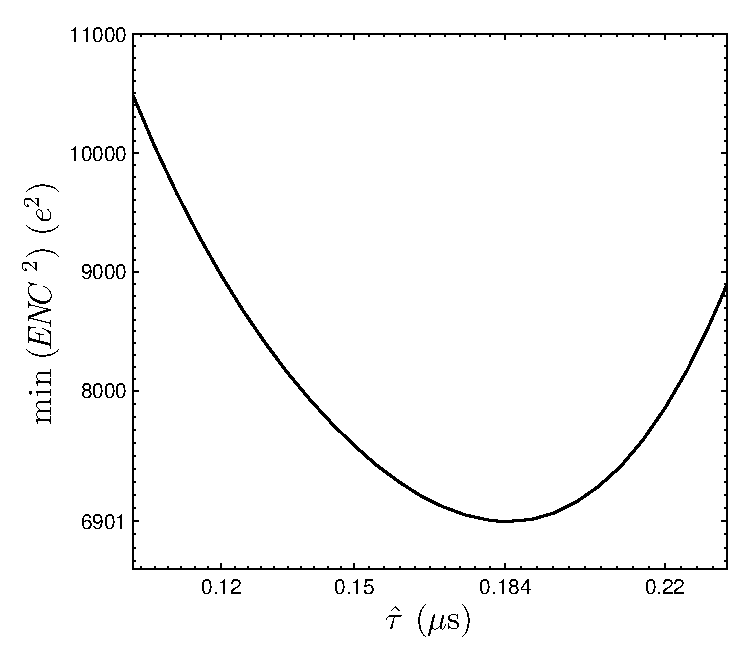
\includegraphics[width=4in]{./Figures/optimum_tau.eps}
	\caption{Minimum $\mathit{ENC}^2$ as a function of $\hat{\tau}$ for a fixed $N$.}\label{fig:optimum_tau}
\end{figure}

\begin{figure}[!t]
	\centering
	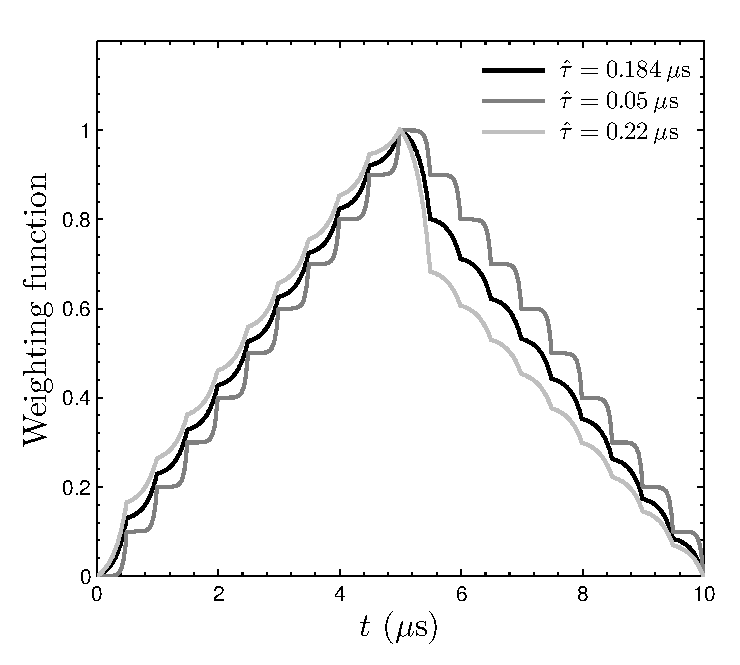
\includegraphics[width=4in]{./Figures/optimum_wf.eps}
	\caption{Optimum WF for different values of $\hat{\tau}$ for $N=20$.}\label{fig:optimum_wf}
\end{figure}

The initial assumption that the filter sampling period $T_s$ is determined by the filter maximum clock rate is only valid if the optimum $\mathit{ENC}^2$ is lower bounded by $T_s$, or equivalently, by $N$. To support this assumption, \figurename~\ref{fig:optimum_N} shows the optimum value of the $\mathit{ENC}^2$ as a function of $N$. Although \figurename~\ref{fig:optimum_N} suggests to use the filter at the maximum clock rate, for a large number of samples the contribution of an additional sample is marginal, thus to determine $N$ other considerations should be taken into account, such as the filter power consumption and the filter design complexity. Additional requirements, such as \mbox{flat-top} or \mbox{zero-area}, can be easily added as constraints in the optimization problem.

\begin{figure}[!t]
	\centering
	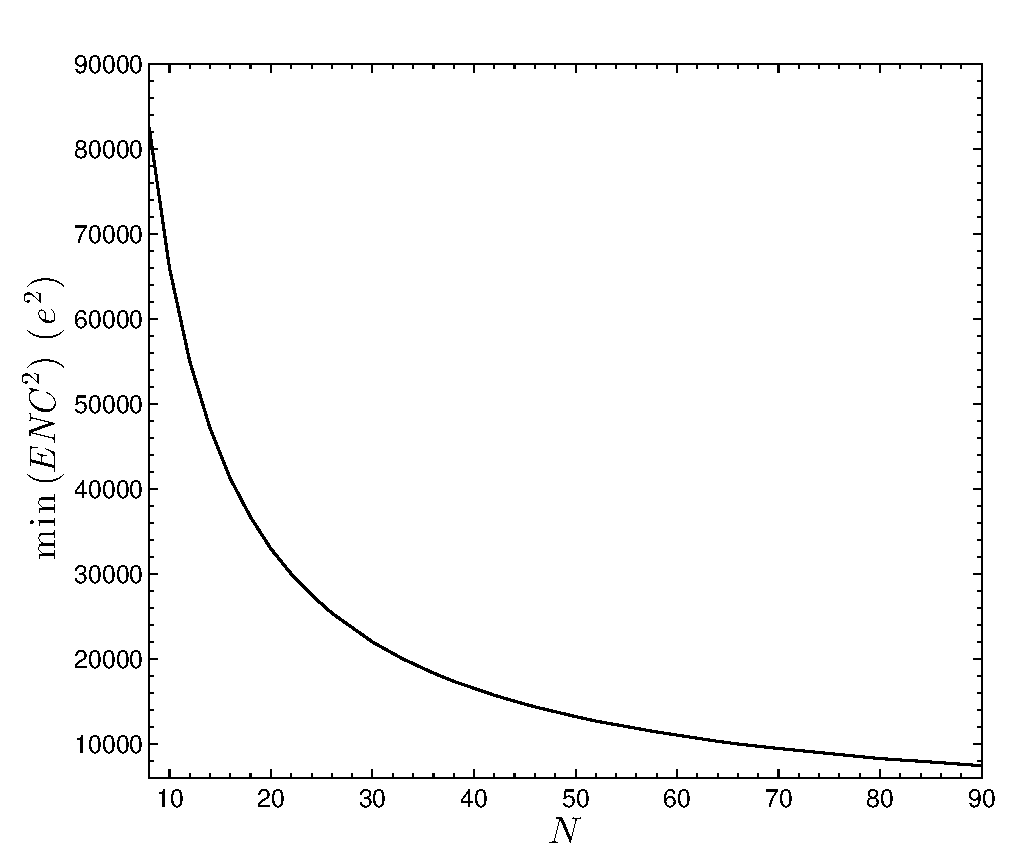
\includegraphics[width=4in]{./Figures/optimum_N.eps}
	\caption{Optimum $\mathit{ENC}^2$ as a function of $N$ for $\hat{\tau} = 0.03\,\mu\text{s}$.}\label{fig:optimum_N}
\end{figure}



%%%%%%%%%%%%%%%%%%%%%%%%%%%%%%%%%%%%%%%%%%%%%%%%%%%%%%%%%%%%%%%%%%%%%%%%%%%%%%
%%%%%%%%%%% SECTION V: CONCLUSION %%%%%%%%%%%%%%%%%%%%%%%%%%%%%%%%%%%%%%%%%%%
%%%%%%%%%%%%%%%%%%%%%%%%%%%%%%%%%%%%%%%%%%%%%%%%%%%%%%%%%%%%%%%%%%%%%%%%%%%%%%
\section{Conclusion}
This work presents a mathematical framework for the analysis of discrete-time filters in the discrete-time domain. The analysis is based on decomposing the total integrated noise at the filter input into a set of discrete-time noise signals, in order to refer them to the filter output and calculate the $\mathit{ENC}$. The proposed analysis only depends on the calculation of the total integrated noise at the filter input, which can be analyzed prior to taking into account the filter itself in order to understand and predict the noise behavior.

In order to validate the proposed framework, the computation of the thermal noise contribution at the output of a \mbox{discrete-time} integrator is presented, and the result is compared to the result produced by the traditional \mbox{continuous-time} approach. Although both methods produce mathematically equivalent results, the former is simpler and more insightful.

This work also presents an example of optimal filter computation, in order to demonstrate the proposed framework capabilities and its application to optimization problems with several noise sources.

\clearpage
\chapter{A SC FILTER FOR ARBITRARY WEIGHTING FUNCTION SYNTHESIS}
\label{chapter:introduction}
\section{Introduction}

%In particle physics experiments, where the results from the collisions are inferred from the measurement of electric charge in various sets of detectors \citep{gatti101,radeka101}, noise sets a fundamental limit for the charge measurement resolution \citep{degeronimo102}. In such experiments, the typical detector \mbox{front-end} circuit comprises a \mbox{charge-sensitive} amplifier (CSA) and a filter, often referred to as pulse shaper. The former is used to convert the input charge signal, coming from the detector electrodes, into a voltage signal, and is responsible for most of the noise present in the readout circuit signal path \citep{degeronimo101,degeronimo102}. The filter is used to convert the voltage signal at the CSA output into a shaped voltage pulse, in order to maximize the \mbox{signal-to-noise} ratio (SNR) at the measurement time.  

%A current trend on particle physics instrumentation is to implement this filter in the discrete time domain, which allows to synthesize weighting functions (WFs) with virtually any shape, producing near-optimum filters. In \citep{diego101} a novel mathematical framework for a design-oriented analysis of discrete-time filters was presented. One of the greatest benefits of this framework is that it allows to easily compute the optimal discrete-time filter that maximize the SNR in a typical detector front-end circuit, a difficult task to achieve using the traditional methods intended for continuous-time networks. In this work, a generic filter designed to be flexible enough to synthesize arbitrary weighting functions is presented, 

One of the greatest benefits of the mathematical framework presented in \citep{avila101} is that it allows to easily find the optimal discrete-time filter that maximizes the SNR of a typical detector front-end circuit, a difficult task to undertake using the traditional methods for continuous-time networks. The filter presented in this chapter is designed to be flexible enough to synthesize arbitrary weighting functions with an adequate resolution. Therefore, it could be used to synthesize the optimal filter described above. The filter is a prototype of the front-end filter for the Bean 2, which was introduced in Chapter~\ref{chapter:problem}. Hence, the main specifications are derived from the Bean specifications. Also, power, noise and size budgets of the referred IC are taken as constraints.

There are two common options for implementing the required filter. The simplest is to digitize the CSA output directly with a fast analog-to-digital converter (ADC)  - $N$ times faster than the typical ADC used, with $N$ the number of desired samples - and then process the samples in the digital domain, whereas the other option is to use a custom \mbox{switched-capacitor} (SC) network as a filter, without changing the ADC requirements. Considering the Bean timing constraints, the former option is not feasible, given that such fast ADC would exceed the available power and size budgets. Hence, the SC solution was chosen.


\section{System-Level Design}
As mentioned in the previous Chapter, to synthesize arbitrary weighting functions the front-end filter should be designed to have a  discrete-time transfer function $F(z)$ given by
\begin{equation}
F(z) = \sum_{j=0}^{N-1}a_{N-j} \hspace{0.1em}z^{-j} \label{eq:filter_tf}
\end{equation}
where $a_i$ are arbitrary coefficients and $N$ is the filter length. Fig.~\ref{fig:filter_post} shows a simplified circuit diagram of a fully-differential SC integrator designed to implement $F(z)$. Some control logic and switches have been purposely omitted.

The filter has two phases of operation. During the sampling phase, $\phi_1$, input voltage charges  both $C_S$ capacitors. During the amplification phase, $\phi_2$, the OTA input virtual short circuit forces charge from capacitors $C_S$ to be transferred to capacitors $C_F$. Thus, at the end of $\phi_2$, the filter output voltage is equal to its value in the previous cycle, plus $C_S V_i/C_F$. Also, an early version of $\phi_1$, $\phi_{1e}$, is used in the sampling phase to implement Bottom-Plate Sampling \citep{haigh101}, a technique used to reduce the charge injection from switches.

In this configuration, the filter instantaneous gain is given by the ratio of the capacitors $C_S$ and $C_F$.  Considering that in order to obtain arbitrary coefficients the filter gain must be programmable, either $C_S$ or $C_F$ should be implemented with a variable capacitor. For simplicity, capacitor $C_S$ was selected for this purpose. The OTA input multiplexers are used to swap the OTA inputs, and therefore, to invert the sign of the filter gain. The OTA output common-mode level is set by the OTA's internal common-mode feedback (CMFB) circuit, whereas the input common-mode level is set by the external reference $V_\textit{icm}$. The OTA output multiplexers are used to bypass the filter for the SDT operation mode and for diagnostic purposes.


\begin{figure}[!t]
	\centering
	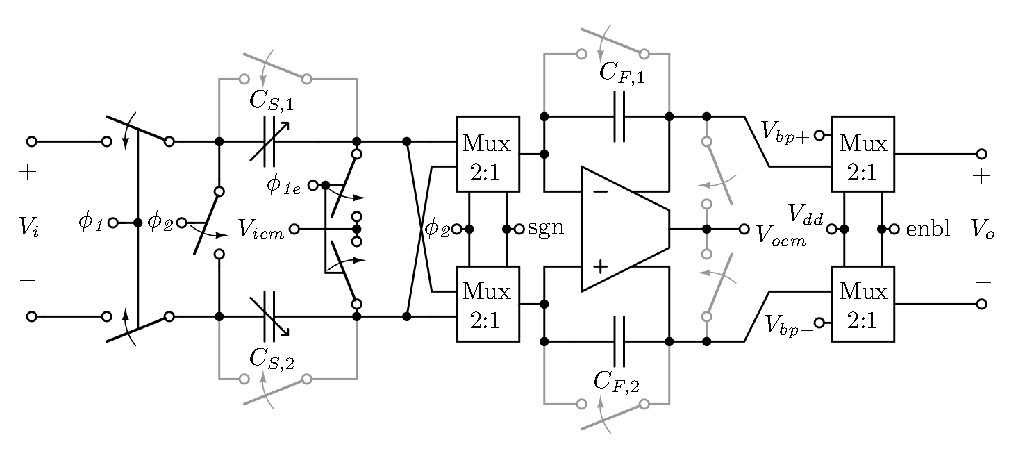
\includegraphics[width=6in]{./Figures/Filter/filter_post.eps}
	\caption{Simplified filter schematic. Reset switches are depicted in gray.}\label{fig:filter_post}
\end{figure}

\subsection{Filter Specifications}

Table \ref{tab:filter_specs} summarizes the filter specifications derived from the Bean specifications (Table \ref{tab:bean_specs}). Also, the CSA output specifications and the ADC input specifications were taken into account. The sampling frequency is $51.95\,\text{MHz}$. Thus, each integration subcycle is $19.25\,\text{ns}$ long. Since each subcycle involves two phases, sampling and holding, each phase has only $9.625\,\text{ns}$ for settling. Considering this time, to assure a dynamic error of $0.1\,\%$ (to meet the dynamic range specification) the amplifier must have an \mbox{unity-gain} frequency of $f_u = 118\,\text{MHz}$ (without considering slew-rate regime). Also, a static error of $0.1\,\%$ is required, which implies an OTA open-loop gain of at least $60\,\text{dB}$. 

\begin{table}[!t]
	\begin{center}
		\begin{tabular}{|l|l|}\hline
			{\bf Specification} & {\bf Value} \\ \hline\hline
			Modes of operation & SDT and DCal \\ \hline
			Input swing & 0.9 V or close \\ \hline
			Output swing & 1 V or close \\ \hline
			Dynamic range & 10 bit \\ \hline
			Gain resolution & 6 bit (7.8 mV/V - 0.5 V/V) \\ \hline
			Noise budget & $1.25\times Q_n^2$ \\ \hline
			Operation speed & $51.95\,\text{MHz}$ \\ \hline
			Power consumption & Minimize\\\hline
		\end{tabular}
		\vspace*{5pt}
		\caption{Filter specifications summary.}\label{tab:filter_specs}
	\end{center}
\end{table}
%Besides the specifications required to implement arbitrary weighting functions, 

%
%In a SC integrator the noise should be analyzed at the two clock phases and then by added
%
%After $N$ integration cycles and assuming an arbitrary $C_S$ at each cycle, the contribution from noise sampled at $\phi_1$ can be computed as
%\begin{equation}
%\overline{V_{\phi_1}^2} = 2 kT \sum_{i=1}^{N} \frac{1}{C_{F_i}}\left(1 + \frac{C_S}{C_{F_i}}\right)
%\end{equation}
%
%In a proper design, switches resistance will be much smaller than $1/\beta g_\textit{m,eff}$, so noise contribution at $\phi_2$ can be assumed dominated by OTA noise. In a one stage OTA
%
%\begin{equation}
%\overline{V_{\phi_2}^2} = \frac{2 N_f kT}{g_\textit{meff}} \sum_{i=1}^{N} \frac{1}{\beta_i C_{Ltot_i}}
%\end{equation}
%
%where $N_f$ is a noise factor dependent on the OTA topology, for a recycling folded cascode
%
%\begin{equation}
%N_f \approx \left(1+\frac{g_{mf}}{g_{meff}}+\frac{g_{ml}}{g_{meff}}\right)
%\end{equation}
%
%
%In a two stage miller compensate OTA the noise is given by (citar a alumno de tom lee, calculo de ruido termico):
%\begin{equation}
%\overline{V_{\textit{filteramp}}^2}\approx 2N\left\{\frac{\gamma}{\beta}\cdot \frac{kT}{C_C}\left(1+\frac{g_{mxx}}{g_{mx}}\right)+\frac{kT}{C_{\textit{Ltot}}}\left[1+\gamma\left(1+\frac{g_{myy}}{g_{my}}\right)\right]\right\}\label{eq:noise_miller_ota}
%\end{equation}
%Where $C_C$ upper bounded by the amplifier speed requirement, looking at the unitary frequency 
%\begin{equation}
%f_u \approx \beta \frac{g_{min}}{2\pi C_C}
%\end{equation}
%
%With $\beta=1$ (worst case scenario), $g_\text{min}$ around a few $mS$ (which is given for a typical OTA solution only considering the gain and frequency requeriments) and considering the restriction for $f_u$, $C_C$ should be around a few hundred of $\textit{fF}$, which replaced in Eq.~\ref{eq:noise_millter_ota} won't complain the noise requirements for the OTA, so a one stage solution should be used.
%
%To obtain enough gain in one stage a folded cascade amplifier is a suitable candidate, using (citar paper de analysis orientado al diseno de ruido), the noise given by a folded cascade ota can be approximated by
%
%\begin{equation}
%\overline{v_{\textit{in}}^2} = \frac{4 \gamma kT}{g_{{min}}} \left(1+y\right)
%\end{equation}
%
%where $y \approx \nicefrac{g_{{mf}}}{g_\text{min}}+\nicefrac{g_{{ml}}}{g_{min}}$, since $g_{mI}$ is larger compared to $1/r_{oL}$ and $1/(r_{oI}\parallel r_{oF})$ the noise contributions of $M_{CF}$ and $M_{CL}$ can be neglected


\section{Circuit Design}
\subsection{Operational Transconductance Amplifier}
The previous version of the Bean uses a two-stage Miller-compensated OTA as the filter amplifier. However, this topology does not lead to a feasible design given the filter specifications, mainly, because of the existing trade-off between noise and bandwidth, resulting from the Miller capacitor. For this version of the Bean, a single stage OTA topology was chosen, as it can theoretically meet the filter specifications.  A folded cascode (FC) OTA would be the first candidate to implement this amplifier, because of its good balance between gain, speed, input-output swing and complexity. Nonetheless, the settling-time specification would require high bias currents due to the slew-rate limitation, which would come into conflict with the power budget. The recycling folded cascode OTA (RFC) \citep{assaad101}, a small variation over the FC OTA, was chosen to overcome this limitation, since it exhibits an enhanced transconductance, gain, and slew-rate (SR) over the conventional FC OTA for the same power and area budgets.

In a traditional FC OTA, folding transistors conduct most of the current and generally have the largest transconductance. However, their role is only limited to providing a folding node for the small signal current \citep{assaad101}. In a RFC OTA (Fig.~\ref{fig:OTA_post}), a small modification over the conventional FC topology allows to use the folding transistors as additional drivers for the small signal input. Therefore, they are used to enhance the effective transconductance of the amplifier. Also, this modification entails additional enhancements over the conventional FC OTA, such as higher and symmetrical SR, higher output resistance and higher crossover-frequency.

In a voltage-controlled voltage source (VCVS), such as the filter amplifier, the low-frequency \mbox{open-loop} gain can be calculated as $|A_V| = G_\textit{m,eff}  \cdot R_\textit{o}$, where $G_\textit{m,eff}$ is the effective transconductance, defined as the ratio of the short-circuit output current to the input voltage, and $R_o$ is the output resistance, defined as the resistance seen at the amplifier output when no input is applied \citep{rashid101}. In a RFC OTA the effective transconductance can be approximated to:
\begin{equation}
G_\textit{m,eff} \approx g_\textit{m,in}(1+K)\label{eq:gmeff}
\end{equation}
where $K$ is the current mirror ratio between transistors $M_f$ and $M_\textit{aux,3}$. Also, the output resistance can be approximated to:
\begin{equation}
R_\textit{o} \approx g_\textit{m,cf}r_\textit{o,cf}\left(r_\textit{o,in}\parallel r_\textit{o,aux3} \right) \parallel g_\textit{m,cl} r_\textit{o,cl} r_\textit{o,l}
\end{equation}

Considering that the RFC OTA is a single-stage amplifier, and assuming a proper design, the dynamic behavior of the open-loop filter will be dominated by the output node resistance and the load capacitance, $C_L$, so other time constants can be ignored. For a RFC OTA, the unity-gain bandwidth, $\omega_u$, is given by:
\begin{equation}
\omega_u = \frac{G_\textit{m,eff}}{C_L}
\end{equation}
Once integrated in the filter, all non-dominant poles and zeros will be beyond the unity-gain frequency. Thus, the closed-loop bandwidth, $\omega_c$, can be approximated to:
\begin{equation}
\omega_c = \beta \frac{G_\textit{m,eff}}{C_\textit{L,tot}}
\end{equation}
where $\beta$ is the feedback factor, given by
\begin{equation}
\beta \approx \frac{C_F}{C_F+C_S+C_\text{parasitic}}
\end{equation}
and $C_\textit{L,tot}$ is the total load capacitance, given by:
\begin{equation}
C_\textit{L,tot} = C_L + (1-\beta)C_F
\end{equation}
where $C_\text{parasitic}$ is the parasitic capacitance at the OTA input node.

In a RFC OTA the SR is symmetrical and enhanced $K$ times over the FC OTA for the same power consumption. Considering $I_\textit{tail}$ as the bias current of the transistor $M_\textit{tail}$, the SR can be computed as:
\begin{equation}
\text{SR} = \frac{2 K I_\textit{tail}}{C_L}
\end{equation}

In a SC integrator, noise is sampled at both clock phases, namely $\phi_1$ and $\phi_2$. Thus, to calculate the filter output-referred total integrated noise, both noise contributions must be calculated separately and added up in quadrature. After $N$ integration cycles and assuming an arbitrary $C_S$ at each cycle, the contribution from noise sampled at $\phi_1$ can be computed as:
\begin{equation}
\overline{V_{\phi_1}^2} = 2 kT \sum_{i=1}^{N} \frac{1}{C_F}\left(1 + \frac{C_{S_i}}{C_F}\right)
\end{equation}
In a proper design, switch resistances will be much smaller than $1/(\beta g_\textit{m,eff})$, so noise at $\phi_2$ can be assumed to be dominated by the OTA noise \citep{vleugels101}. Thus, the noise contribution at $\phi_2$ can be approximated to:
\begin{equation}
\overline{V_{\phi_2}^2} \approx \frac{2 N_f kT\gamma}{g_\textit{m,eff}} \sum_{i=1}^{N} \frac{1}{\beta_i C_{Ltot_i}}
\end{equation}
where $N_f$ is a noise factor dependent on the single-stage OTA topology, for a RFC:
\begin{equation}
N_f \approx \frac1{1+K}\left(\frac{1+K^2}{1+K} + \frac{g_\textit{m,f}}{g_\textit{m,in}} + \frac1{1+K}\frac{g_\textit{m,l}}{g_\textit{m,in}}\right) \label{eq:Nf}
\end{equation}
Table~\ref{tab:OTA_sizes} shows the parameter values for the OTA design. Transistor sizes were calculated using equations \ref{eq:gmeff} to \ref{eq:Nf} and a semi-exhaustive search script, with tabulated pre-simulated data and using the $g_m/I_D$ design technique \citep{silveira101}. Computational power was not a problem at this point. However, for a deeper optimal design, a bigger domain must be chosen (not increasing the boundaries but increasing the domain resolution) and an intelligent algorithm must be used, e.g like the use of Support Vector Machines in \citep{bernardinis101} to filter the feasible domain of solutions.
\begin{figure}[!t]
	\centering
	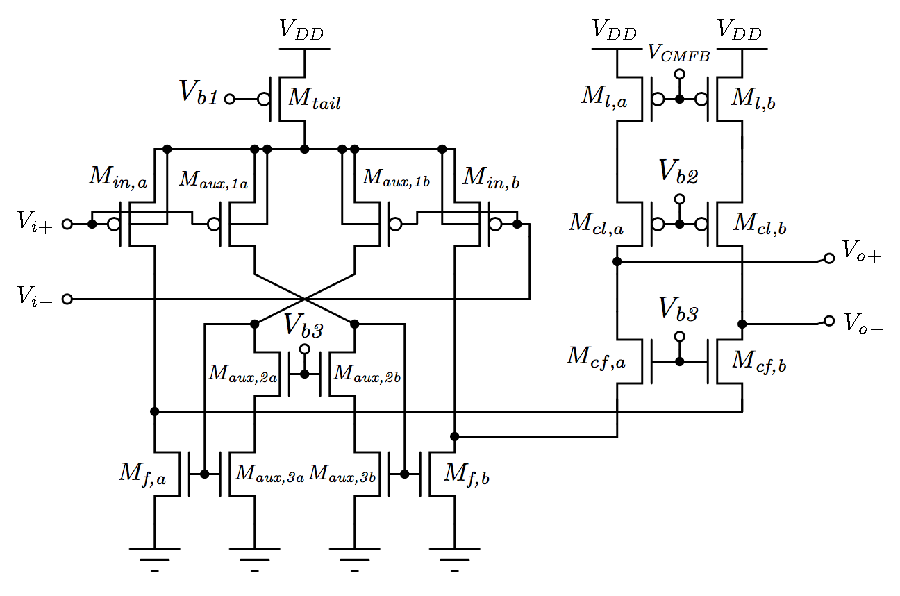
\includegraphics[width=5.5in]{./Figures/Filter/OTA_post.eps}
	\caption{Recycling folded cascode OTA schematic. Three terminal NMOS and PMOS devices are with their bodies tied to ground and $V_\textit{DD}$ respectively.}\label{fig:OTA_post}
\end{figure}
\begin{figure}[!t]
	\centering
	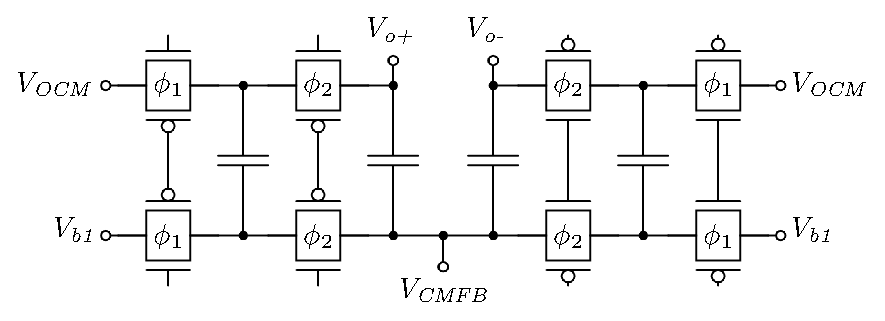
\includegraphics[width=4.6in]{./Figures/Filter/CMFB_post.eps}
	\caption{OTA discrete-time commmon-mode feedback circuit schematic.}\label{fig:CMFB_post}
\end{figure}
\begin{figure}[!t]
	\centering
	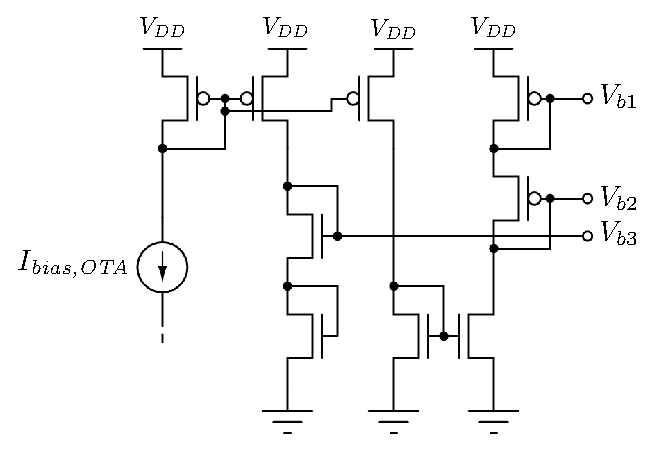
\includegraphics[width=4in]{./Figures/Filter/bias_ota_post.eps}
	\caption{OTA bias network schematic.}\label{fig:bias_ota_post}
\end{figure}
\begin{table}[!t]
	\begin{center}
		\begin{tabular}{|l|r|r|r|r|}\hline
			Transistor & Bias current & $g_m/I_D$ & $W$ & $L$ \\ \hline\hline
			$M_\text{in}$ & $51.3\,\mu\text{A}$  & $14.9\,\text{mS}/\text{mA}$  & $48\,\mu\text{m}$ & $0.36\,\mu\text{m}$ \\ \hline
			$M_\text{tail}$ & $201.7\,\mu\text{A}$  & $8.2\,\text{mS}/\text{mA}$  & $64\,\mu\text{m}$ & $0.45\,\mu\text{m}$ \\ \hline 
			$M_\text{f}$ & $100.6\,\mu\text{A}$  & $8.7\,\text{mS}/\text{mA}$  & $8\,\mu\text{m}$ & $0.45\,\mu\text{m}$ \\ \hline
			$M_\text{cf}$ & $49.3\,\mu\text{A}$  & $11.7\,\text{mS}/\text{mA}$  & $8\,\mu\text{m}$ & $0.45\,\mu\text{m}$ \\ \hline
			$M_\text{cl}$ & $49.3\,\mu\text{A}$  & $10.7\,\text{mS}/\text{mA}$  & $16\,\mu\text{m}$ & $0.3\,\mu\text{m}$ \\ \hline
			$M_\text{l}$ & $49.3\,\mu\text{A}$  & $7.6\,\text{mS}/\text{mA}$  & $32\,\mu\text{m}$ & $1\,\mu\text{m}$ \\ \hline
			$M_\text{aux,1}$ & $49.6\,\mu\text{A}$  & $15\,\text{mS}/\text{mA}$  & $48\,\mu\text{m}$ & $0.36\,\mu\text{m}$ \\ \hline
			$M_\text{aux,2}$ & $49.6\,\mu\text{A}$  & $9.5\,\text{mS}/\text{mA}$  & $2\,\mu\text{m}$ & $0.18\,\mu\text{m}$ \\ \hline
			$M_\text{aux,3}$ & $49.6\,\mu\text{A}$  & $6\,\text{mS}/\text{mA}$  & $4\,\mu\text{m}$ & $0.45\,\mu\text{m}$ \\ \hline
		\end{tabular}
		\vspace*{5pt}
		\caption{Filter OTA design values.}
		\label{tab:OTA_sizes}
	\end{center}
\end{table}

\subsection{Variable Capacitor}
Fig.~\ref{fig:cap_array_post} shows a schematic of the binary-weighted array used to implement the variable capacitor $C_S$. All capacitors $C_{S,bn}$ were designed as a parallel connection of unit MIM capacitors $C_u=8.1\,\text{fF}$  (with an area of $2.7\,\micro\text{m}\times2.7\,\micro\text{m}$), which for matching purposes were also used to implement capacitor $C_F$. CMOS switches were sized to meet filter speed specifications.  Switch control signals will be directly bonded out off-chip. A \mbox{serial-programmable} memory to store the filter coefficients, and which will be connected directly to these control signals - to avoid the \mbox{unnecessary} use of IC pads -, will be included in future revisions of the Bean.

\begin{figure}[!t]
	\centering
	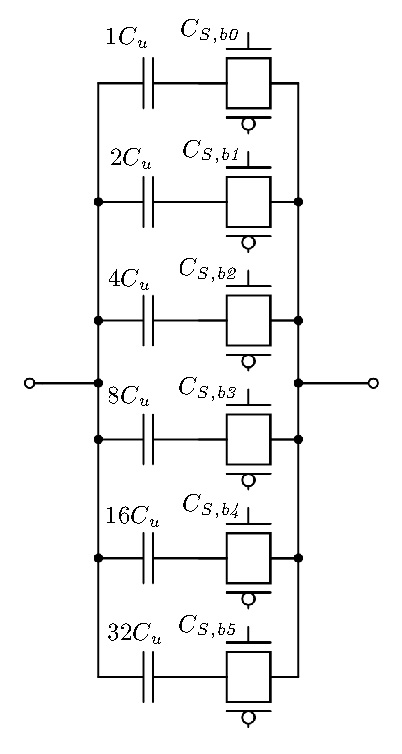
\includegraphics[width=1.8in]{./Figures/Filter/cap_array_post.eps}
	\caption{6-bit programmable capacitor.}\label{fig:cap_array_post}
\end{figure}

\subsection{Rail-to-Rail buffer}
A signal buffer is required to buffer some of the Bean prototype voltages for scope probing. The buffer must be able to drive a $8\,\text{pF}$ load at a reasonable speed and power dissipation, with truly rail-to-rail input and output voltages. Fig.~\ref{fig:buffer_post} shows the schematic of a rail-to-rail operational amplifier (op-amp) used to implement a unity gain voltage buffer amplifier.

The two-stage op-amp consists of a rail-to-rail constant-$g_m$ input stage \citep{hogervorst101}, composed by two complementary input pairs and an electronic zener diode, $M_\text{in1}$-$M_\text{in2}$, $M_\text{ip,a}$-$M_\text{ip,b}$ and $M_\textit{zp}$-$M_\textit{zn}$,  followed by folded-cascode, current-mirroring loads, \mbox{$M_\textit{cln1}$-$M_\textit{ln1}$}, $M_\textit{cln2}$-$M_\textit{ln2}$, $M_\textit{clp1}$-$M_\textit{lp1}$ and $M_\textit{clp2}$-$M_\textit{lp2}$, and a class-AB output \citep{hogervorst102}, $M_\textit{op}$-$M_\textit{on}$. Transistors $M_\textit{sn1}$-$M_\textit{sn2}$ and $M_\textit{sp1}$-$M_\textit{sp2}$ implement a translinear loop \citep{analogessentials}, producing the voltage shifts necessary to set the output devices quiescent current consumption.

As for most of two-stage amplifiers, stability must be assured with a proper compensation scheme. In this design, capacitor $C_C$, also known as Miller capacitor, is placed to lower the frequency of the dominant pole and to increase the frequency of the secondary pole, and thus, it helps to increase the phase margin of the amplifier, while resistor $R_Z$ is used to cancel the right-half plane zero that appears because adding $C_C$. Since $C_C$ is calculated as a function of the input stage's total transconductance, the constant-$g_m$ compensation technique used for the input stage helps to maintain a constant frequency response over all the input common mode range.

To assure predictable bias currents and a true rail-to-rail input and output voltage ranges, a proper bias network must be designed. Fig.~\ref{fig:bias_buffer_post} shows a schematic of the bias network used for this op-amp \citep{baker101}. All bias voltages are driven by cascoded current mirrors, which have high output resistance in order to reduce the influence of $V_{ds}$ over the mirrored current. Transistor sizes were calculated to assure  a maximum amplifier output swing and mirrors currents were chosen to maintain a good tradeoff between mirrored currents sensibility and bias network power consumption. 

Table~\ref{tab:buffer_sizes} shows the parameter values for the rail-to-rail buffer design, transistor sizes were calculated with the same methodology as for the OTA design. SPICE simulations predict an open-loop DC gain of $103$\,dB, a crossover frequency of $52$,MHz, and a phase margin of $78\,^\circ$ measured with an $8\,\text{pF}$ load. 
\begin{table}[!t]
	\begin{center}
		\begin{tabular}{|l|r|r|r|r|}\hline
			Transistor & Bias current & $g_m/I_D$ & $W$ & $L$ \\ \hline\hline
			$M_\textit{in}$ & $10.4\,\mu\text{A}$ & $21.2\,\text{mS}/\text{mA}$ & $12.8\,\mu\text{m}$ & $0.45\,\mu\text{m}$ \\ \hline
			$M_\textit{ip}$ & $9.2\,\mu\text{A}$ & $19.4\,\text{mS}/\text{mA}$ & $40\,\mu\text{m}$ & $0.45\,\mu\text{m}$ \\ \hline
			$M_\textit{tp}$ & $60.6\,\mu\text{A}$ & $7.4\,\text{mS}/\text{mA}$ & $20\,\mu\text{m}$ & $0.45\,\mu\text{m}$ \\ \hline
			$M_\textit{tn}$ & $62.9\,\mu\text{A}$ & $9.2\,\text{mS}/\text{mA}$ & $6.4\,\mu\text{m}$ & $0.45\,\mu\text{m}$ \\ \hline
			$M_\textit{lp}$ & $26.3\,\mu\text{A}$ & $9.1\,\text{mS}/\text{mA}$ & $10\,\mu\text{m}$ & $0.45\,\mu\text{m}$ \\ \hline
			$M_\textit{clp}$ & $16\,\mu\text{A}$ & $14.2\,\text{mS}/\text{mA}$ & $20\,\mu\text{m}$ & $0.45\,\mu\text{m}$ \\ \hline
			$M_\textit{ln}$ & $25.2\,\mu\text{A}$ & $10.9\,\text{mS}/\text{mA}$ & $3.2\,\mu\text{m}$ & $0.45\,\mu\text{m}$ \\ \hline
			$M_\textit{cln}$ & $16\,\mu\text{A}$ & $16.8\,\text{mS}/\text{mA}$ & $6.4\,\mu\text{m}$ & $0.45\,\mu\text{m}$ \\ \hline
			$M_\textit{op}$ & $282\,\mu\text{A}$ & $9\,\text{mS}/\text{mA}$ & $100\,\mu\text{m}$ & $0.45\,\mu\text{m}$ \\ \hline
			$M_\textit{on}$ & $282\,\mu\text{A}$ & $10.7\,\text{mS}/\text{mA}$ & $32\,\mu\text{m}$ & $0.45\,\mu\text{m}$ \\\hline
		\end{tabular}
		\vspace*{5pt}
		\caption{Rail-to-rail buffer main design values.}
		\label{tab:buffer_sizes}
	\end{center}
\end{table}
\begin{figure}[!t]
	\centering
	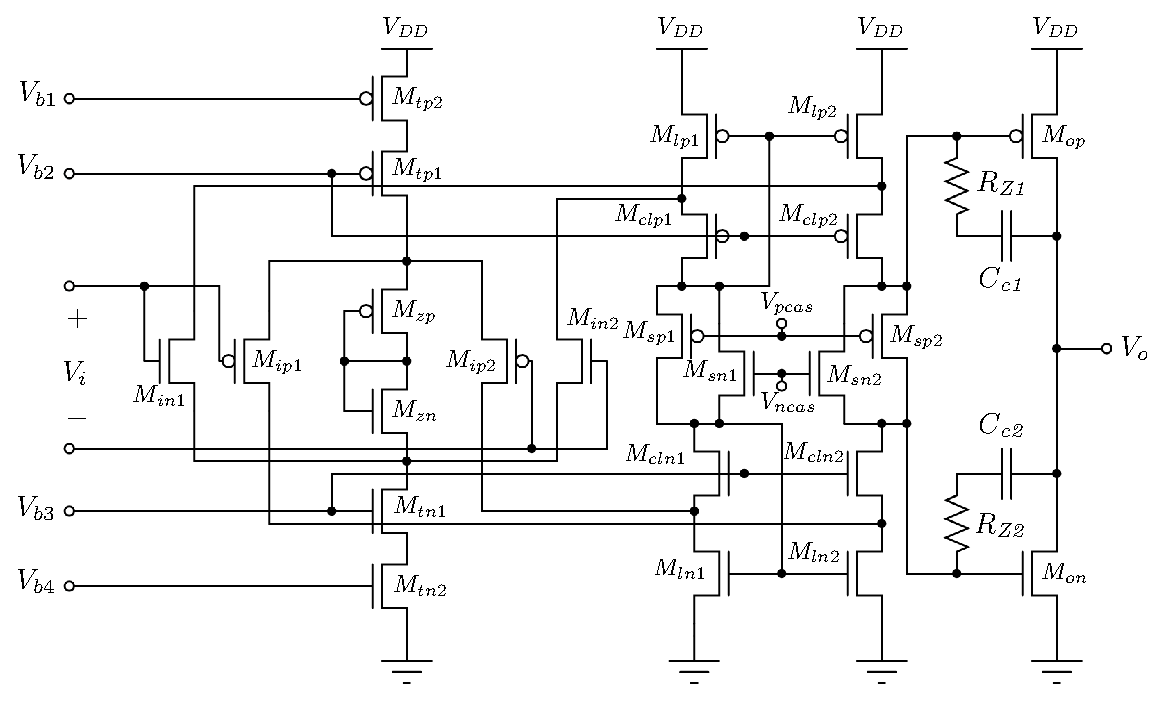
\includegraphics[width=6in]{./Figures/Filter/buffer_post.eps}
	\caption{Rail-to-rail operational amplifier schematic.}\label{fig:buffer_post}
\end{figure}
\begin{figure}[!t]
	\centering
	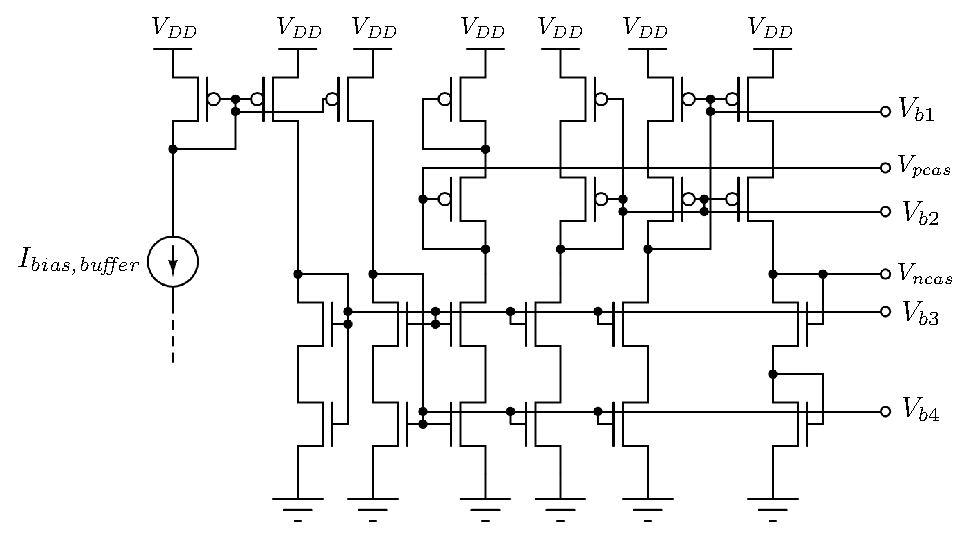
\includegraphics[width=5in]{./Figures/Filter/bias_buffer_post.eps}
	\caption{Op-amp bias network schematic.}\label{fig:bias_buffer_post}
\end{figure}


\subsection{IC bias network}
The previous version of the Bean uses a voltage distribution scheme to bias all the circuits on the IC, but it can cause big problems due to IR drop and process gradients, so a more common current distribution scheme was chosen for this design iteration \citep{murmann101}.  Main disadvantage of this architecture is the additional current consumption, but this drawback is marginal compared to the entire IC power budget and the obtained benefits. To achieve a good power supply rejection (PSR), a supply-insensitive bias network was chosen to implement the global bias cell, from which all the bias currents are generated. Fig.~\ref{fig:bias_all_post} shows a diagram of the current distribution bias scheme. For simplicity, only three current branches are illustrated, although five were used in the final design. Fig.~\ref{fig:bias_filter_post} shows a schematic of a $\beta$-multiplier bias circuit, the architecture selected to implement the supply-insensitive bias network. This consist of a \mbox{self-biased} \mbox{current-reference} network, a \mbox{start-up} circuit, because there are two possible operating points, and a cascode current mirror. The $\beta$-multiplier is an example of a circuit that uses positive feedback. The addition of the resistor kills the closed loop gain\footnote{A positive feedback system can be stable if its closed loop gain is less than one.}. However, if the parasitic capacitance of this resistor is large, it will increase the loop gain and push the feedback system closer to instability. If the resistor, for example, is bonded out off-chip to set the current, it is likely that this bias circuit will oscillate \citep{baker101}.

\begin{figure}[!t]
	\centering
	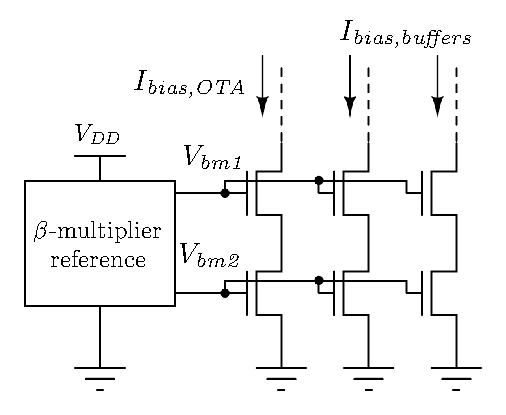
\includegraphics[width=3in]{./Figures/Filter/bias_all_post.eps}
	\caption{Current distribution bias scheme.}\label{fig:bias_all_post}
\end{figure}
\begin{figure}[!t]
	\centering
	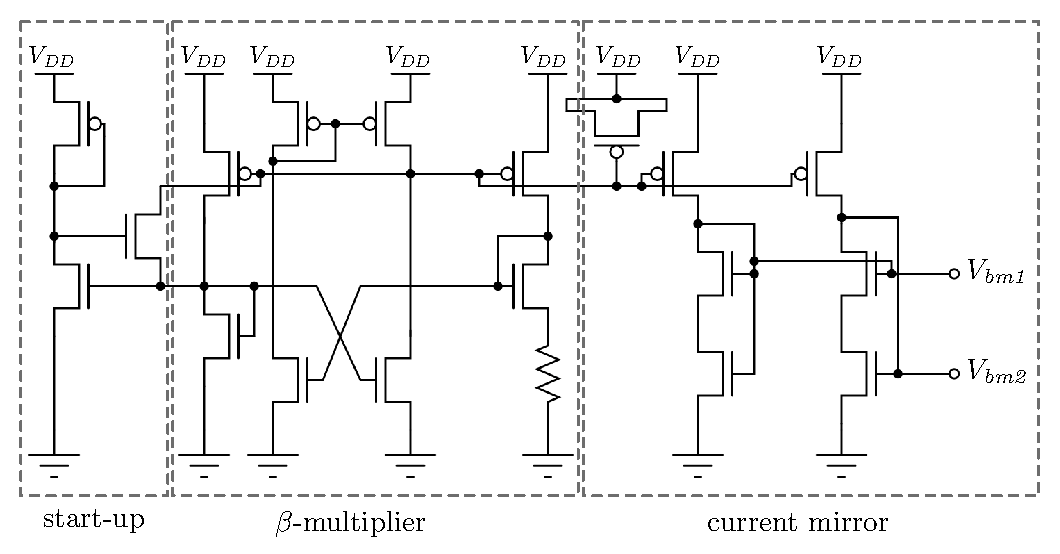
\includegraphics[width=6in]{./Figures/Filter/bias_filter_post}
	\caption{$\beta$-multiplier bias schematic.}\label{fig:bias_filter_post}
\end{figure}
\clearpage
\chapter{RESULTS}
\label{chapter:results}

\section{The Bean V2 prototype Implementation}
The Bean V2 prototype was designed for a standard mixed-signal 180-nm CMOS process. This iteration of the Bean includes two standalone structures: a trimmed version a readout channel, which includes two CSA (one with its input and output shorted to generate the baseline voltage\footnote{The baseline is defined as the CSA DC output voltage after reset, when no input has been applied.}), a pre-charger circuit, the designed SC filter and output buffers; and an isolated version of the filter with its inputs directly bonded out off-chip.  Both structures will be tested separately, thus control signals and reference voltages for both filters are tied together. Also, a logic circuit to generate the non-overlapping two-phase clock was included. Future revisions of the Bean will include an ADC within the channel.

Fig.~\ref{fig:IC_layout} shows the layout of the Bean V2 prototype; for a detailed description of the IC pinout, see Appendix~A. Each channel cell was designed to have a pitch lower than $190\,\mu\text{m}$. If the number of channels is increased to the nominal value of 32, the IC will be approximately 6~mm tall, which can be fit into four mini@sic sub-blocks according to the Europractice rules. After including the ADC and the digital memory, channel length is expected to be lower than $1\,\text{mm}$.

The SC filter, shown in Fig.~\ref{fig:filter_layout}, has a total area of $185\,\mu\text{m}\times 332\,\mu\text{m}$, and was layout to resemble the components spatial distribution of circuit in Fig.~\ref{fig:filter_post}. The filters outputs, the main CSA output and the baseline voltage are buffered out off-chip using the rail-to-rail amplifiers (connected as unity-gain buffers) shown in Fig.~\ref{fig:buffer_layout}. The CSA and the filter OTA are depicted in Figs.~\ref{fig:csa_layout} and \ref{fig:ota_layout} respectively. All structures were carefully side-shielded with multiple guard-rings. Also, to mitigate the effects of cross-chip gradients,  common-centroid technique and dummy devices were used in the layout of the filter OTA and the rail-to-rail op-amps. These considerations were not taken into account for the CSA layout, since mismatch is not critical for this cell because of the size of its transistors and because it is single-ended. As mentioned in the previous chapter, $C_F$ and $C_S$ capacitors were implemented with a parallel connection of unity capacitors. To prevent copper-dishing effects, both capacitors were surrounded by dummy capacitors implemented with the same unity capacitors.

Because of the lack of models for the pads provided by Faraday and the tools needed to use them, it was necessary to design custom pads. They were designed for ground, positive supply voltage, analog input/output, digital input, and digital output. Special care was taken for the Latch-up failure of the output digital drivers, and the Electrostatic discharge phenomena. 


\begin{figure}[!t]
	\centering
	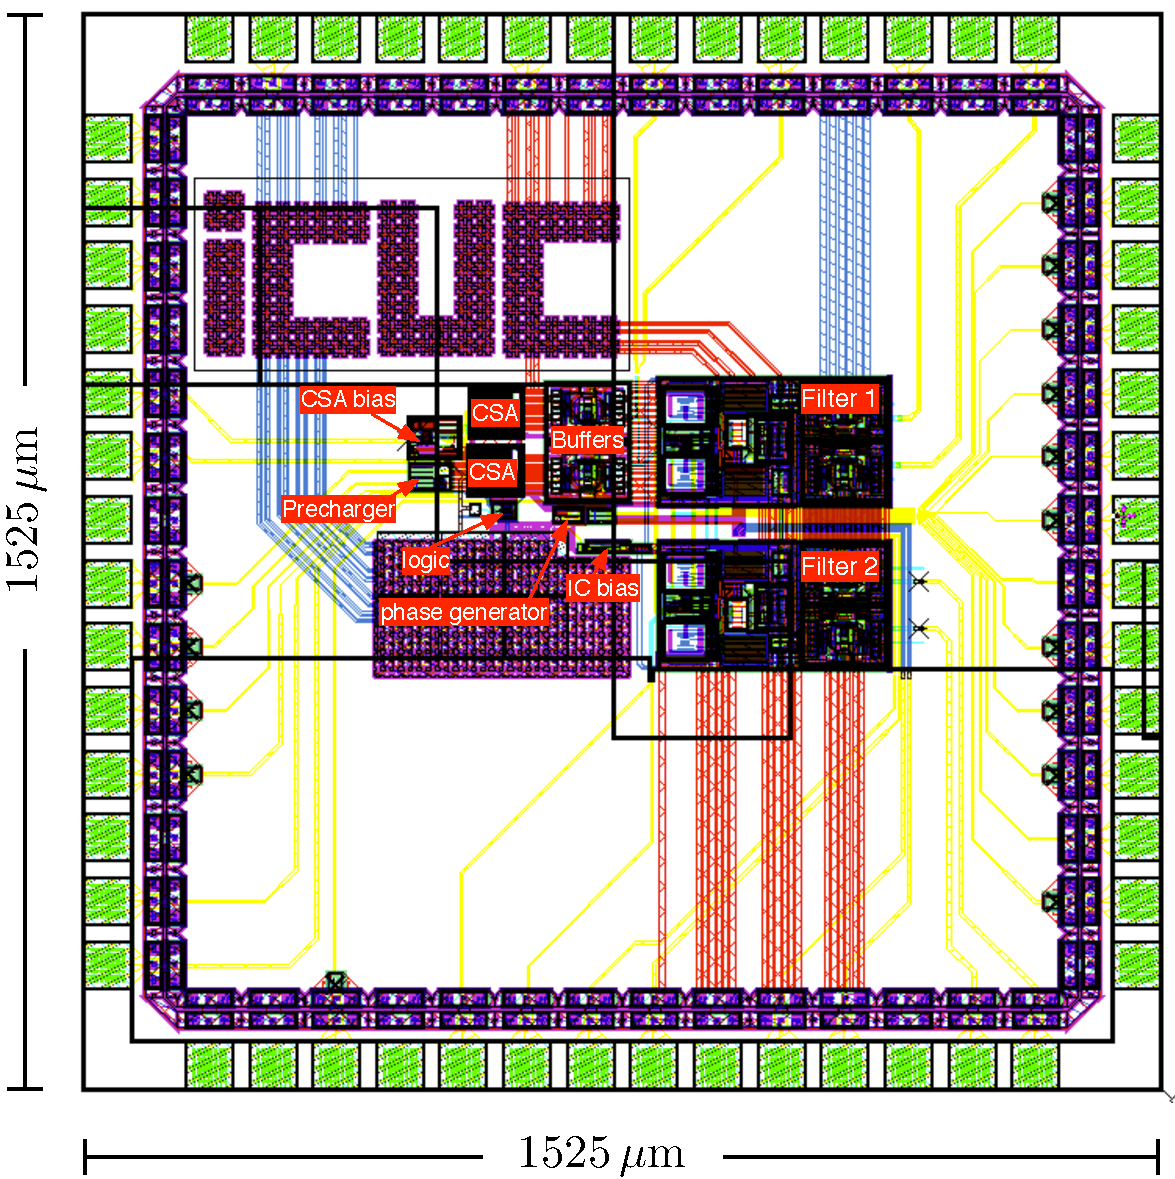
\includegraphics[width=5in]{./Figures/IC_layout}
	\caption{The Bean 2 prototype layout.}\label{fig:IC_layout}
\end{figure}


\begin{figure}[!t]
	\centering
	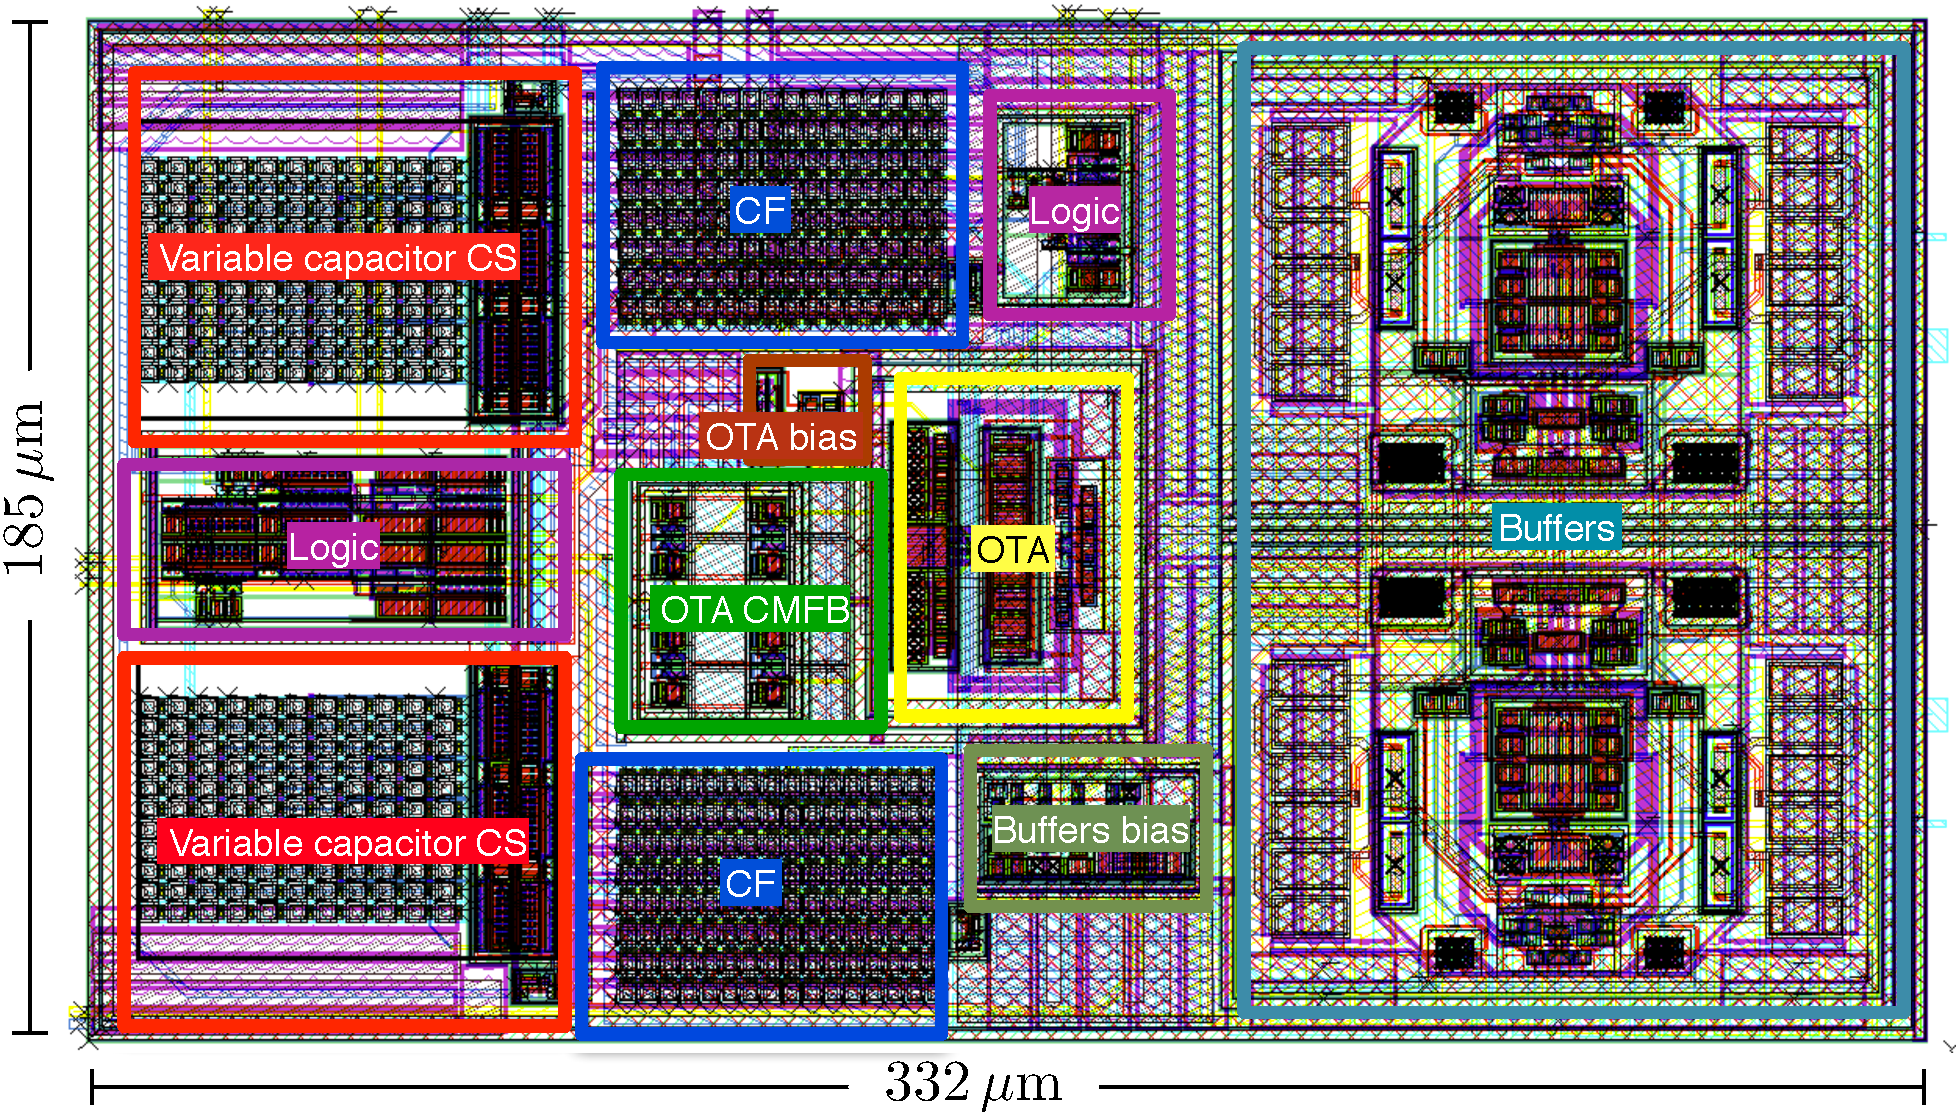
\includegraphics[width=6in]{./Figures/filter_layout}
	\caption{Filter Layout.}\label{fig:filter_layout}
\end{figure}


\begin{figure}[!p]
	\centering
	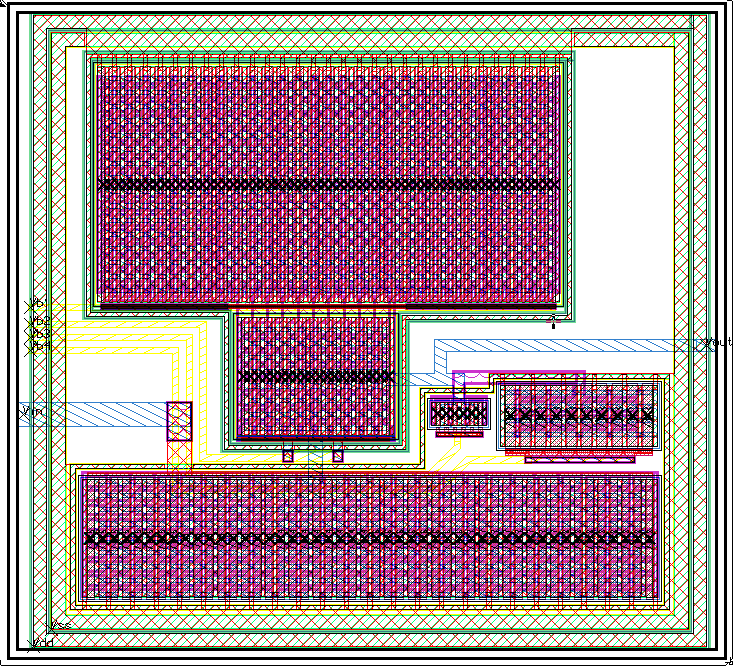
\includegraphics[width=4in]{./Figures/CSA_layout}
	\caption{Charge-sensitive amplifier layout.}\label{fig:csa_layout}
\end{figure}

\begin{figure}[!t]
	\centering
	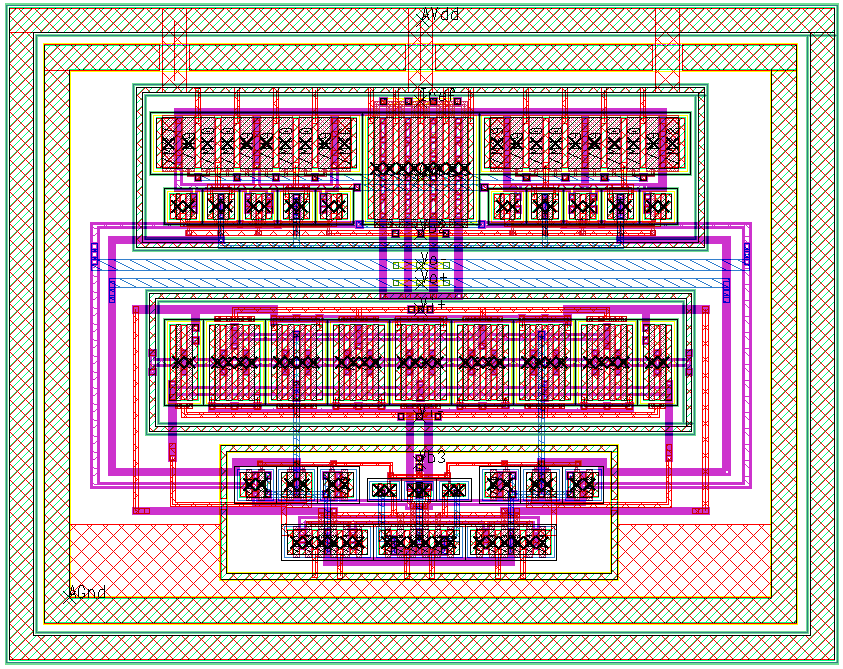
\includegraphics[width=4.5in]{./Figures/OTA_layout}
	\caption{Recycling folded cascode OTA layout.}\label{fig:ota_layout}
\end{figure}

\begin{figure}[!t]
	\centering
	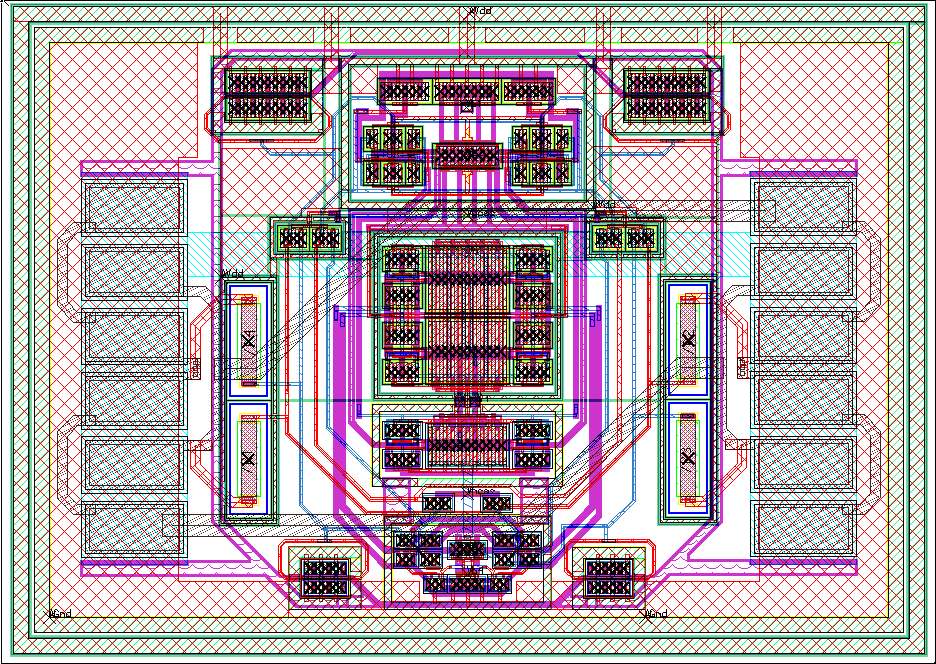
\includegraphics[width=4.5in]{./Figures/buffer_layout}
	\caption{Rail-to-rail operational amplifier layout.}\label{fig:buffer_layout}
\end{figure}


\section{Filter post-layout simulation results}
\subsection{Sub-blocks}
The filter OTA and the buffer op-amp are the complex sub-blocks of the design. Thus, before proceeding with the complete layout,  both structures were separately extracted and individually simulated. Figs.~\ref{fig:bode_OTA} and \ref{fig:bode_buffer}  shows the simulated open-loop response of the filter OTA and the buffer op-amp respectively. Proper 

\begin{figure}[!t]
	\centering
	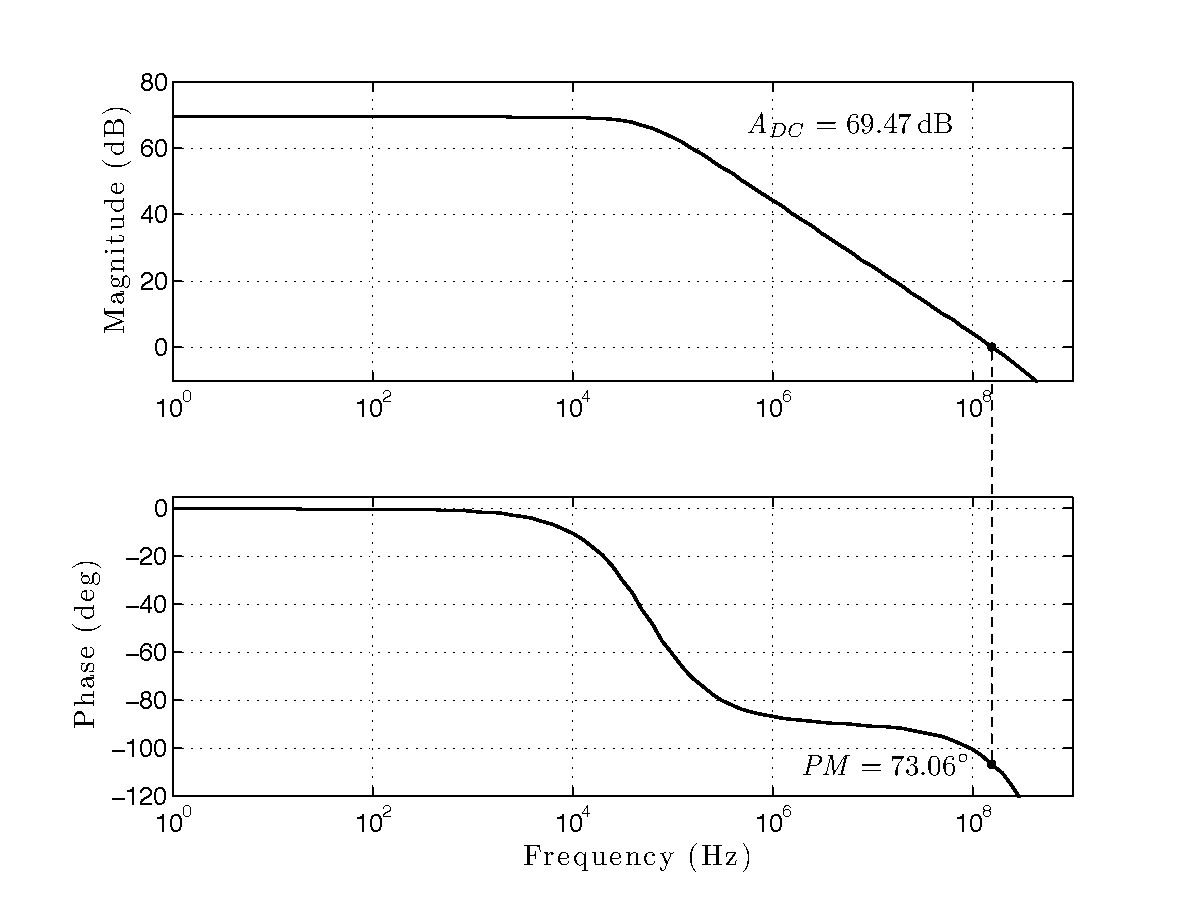
\includegraphics[width=5.3in]{./Test/bode_OTA_post}
	\caption{Bode plot for the OTA open-loop response.}\label{fig:bode_OTA}
\end{figure}

\begin{figure}[!t]
	\centering
	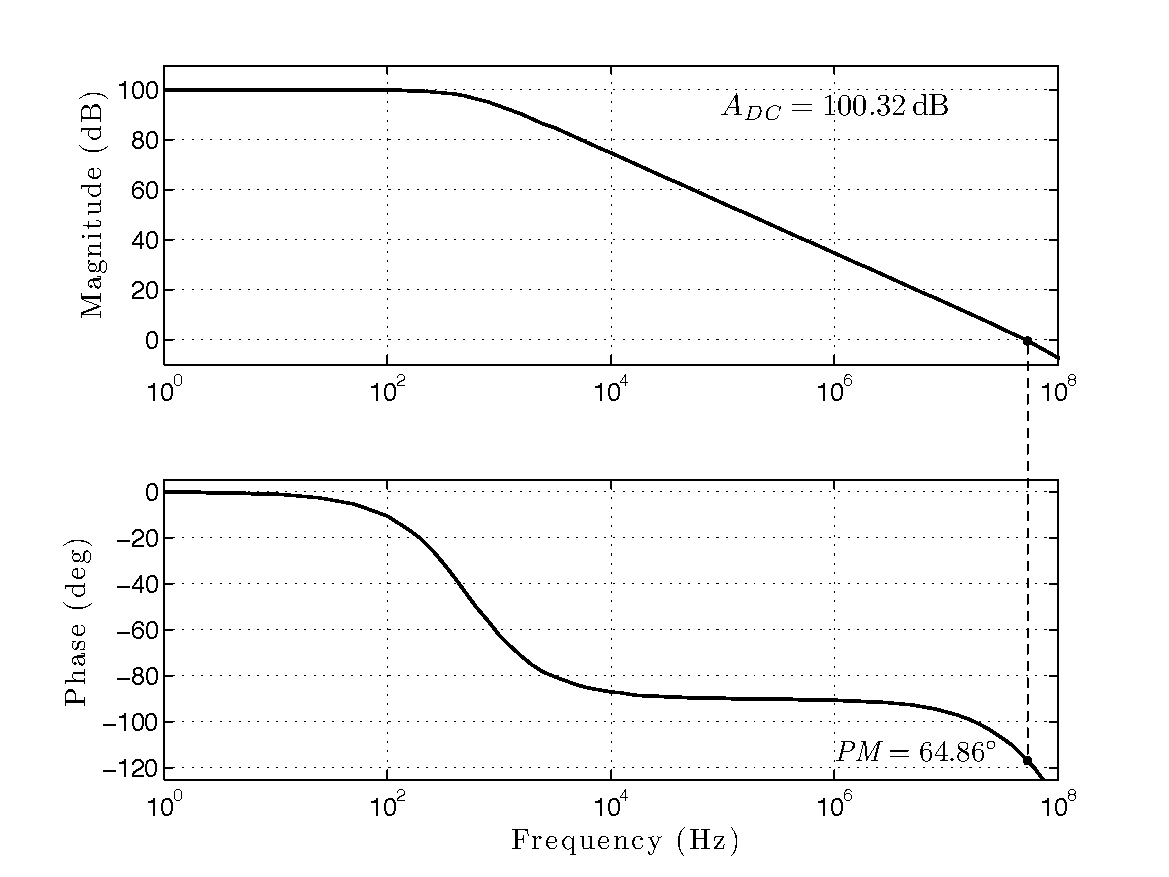
\includegraphics[width=5.3in]{./Test/bode_buffer_post}
	\caption{Bode plot for the buffer open-loop response.}\label{fig:bode_buffer}
\end{figure}

\subsection{Power dissipation} 

The power dissipated by the SC filter prototype was calculated using transient simulations over the extracted filter, under nominal operation and a single input value. The results are presented in Table~\ref{tab:power_dissipation}, the measurements are current consumption averages of the supply node of each component. 

\begin{table}
	\begin{center}
		\begin{tabular}{|l|c|}\hline
			{\bf Component} & {\bf Current dissipation} \\ \hline\hline
			%CSA & $2.718\,\text{mW}$ \\ \hline			
			%CSA bias & $0.954\,\text{mW}$ \\ \hline			 
			Filter OTA & $369\,\mu\text{A}$ \\ \hline
			Filter bias and logic & $194\,\mu\text{A}$ \\ \hline
			Unitary-gain buffer & $360\,\mu\text{A}$ \\ \hline
		\end{tabular}
		\vspace*{5pt}
		\caption{SC filter simulated current dissipation.}
		\label{tab:power_dissipation}
	\end{center}
\end{table}


\subsection{Functionality} 
\subsection{Linearity}
\subsection{Weighting function}
The filter weighting function (WF) was measured according to its definition described in Chapter~\ref{chapter:theoretical}. This was done by applying an input voltage step at different times within a cycle, and measuring the output at the measurement time. A simple $RC$ network was used to simulate a realistic voltage step. Fig.~\ref{fig:wf_test_circuit} shows the circuit used to perform this measurement. 

Fig.~\ref{fig:sim_wf} shows the post-layout SPICE-simulated WF of the filter using plain coefficients and the Bean nominal clock frequency. As expected its shape resembles the shape of the WFs in Fig.~\ref{fig:optimum_wf}. Although the filter exceeds the settling time specification, 

 As explained before, the filter does not reach required settling time 

\begin{figure}[!t]
	\centering
	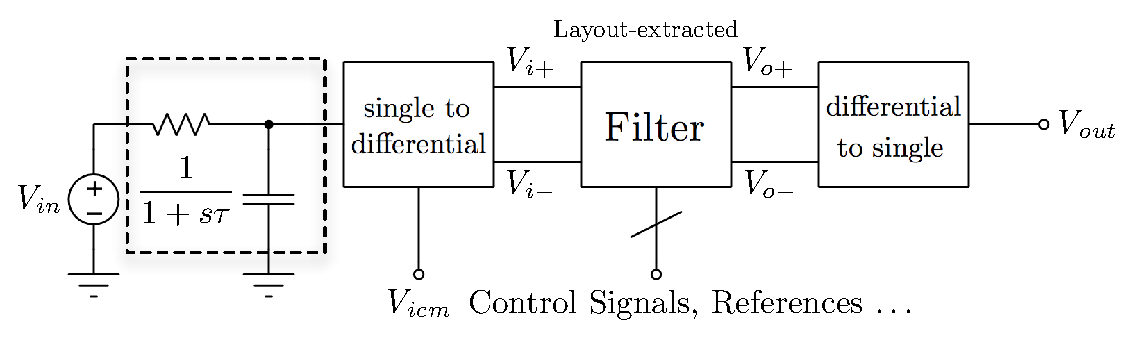
\includegraphics[width=5in]{./Test/wf_test_circuit}
	\caption{Weighting function test circuit.}\label{fig:wf_test_circuit}
\end{figure}

\begin{figure}[!t]
	\centering
	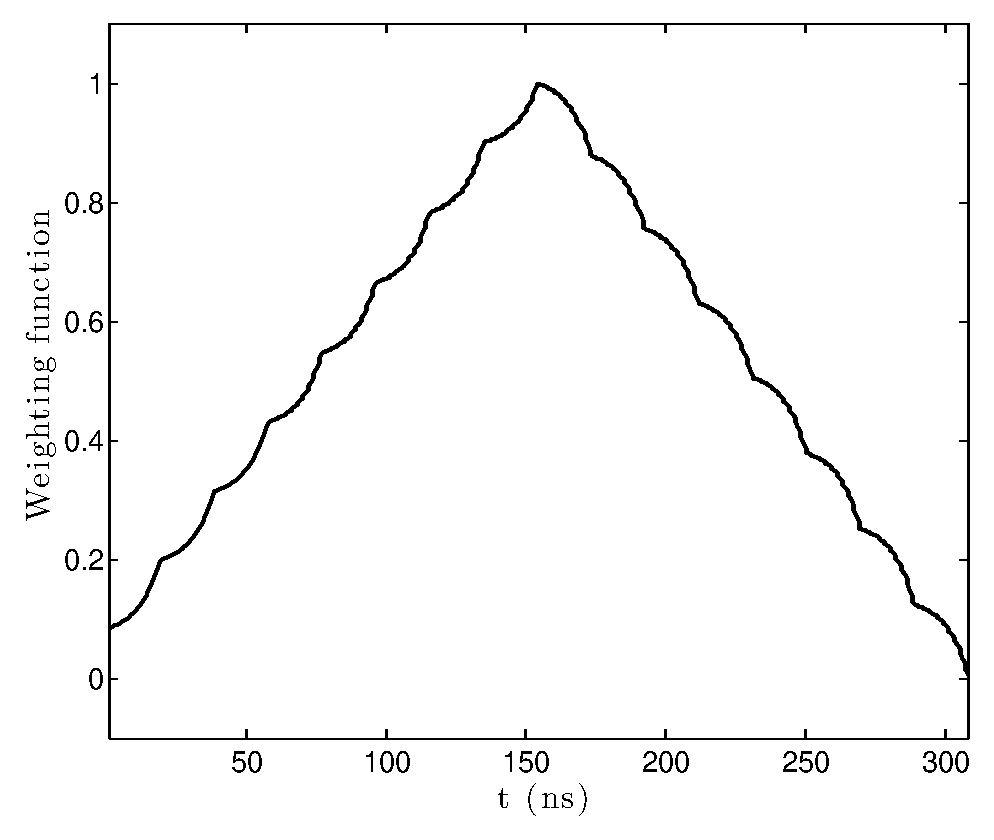
\includegraphics[width=3.6in]{./Test/sim_wf}
	\caption{SPICE-simulated weighting function. $\tau=8\,\text{ns}$, $N=16$ and $T_s=19.25\,\text{ns}$.}\label{fig:sim_wf}
\end{figure}

To characterize the designed filter and 
\begin{figure}[!t]
	\centering
	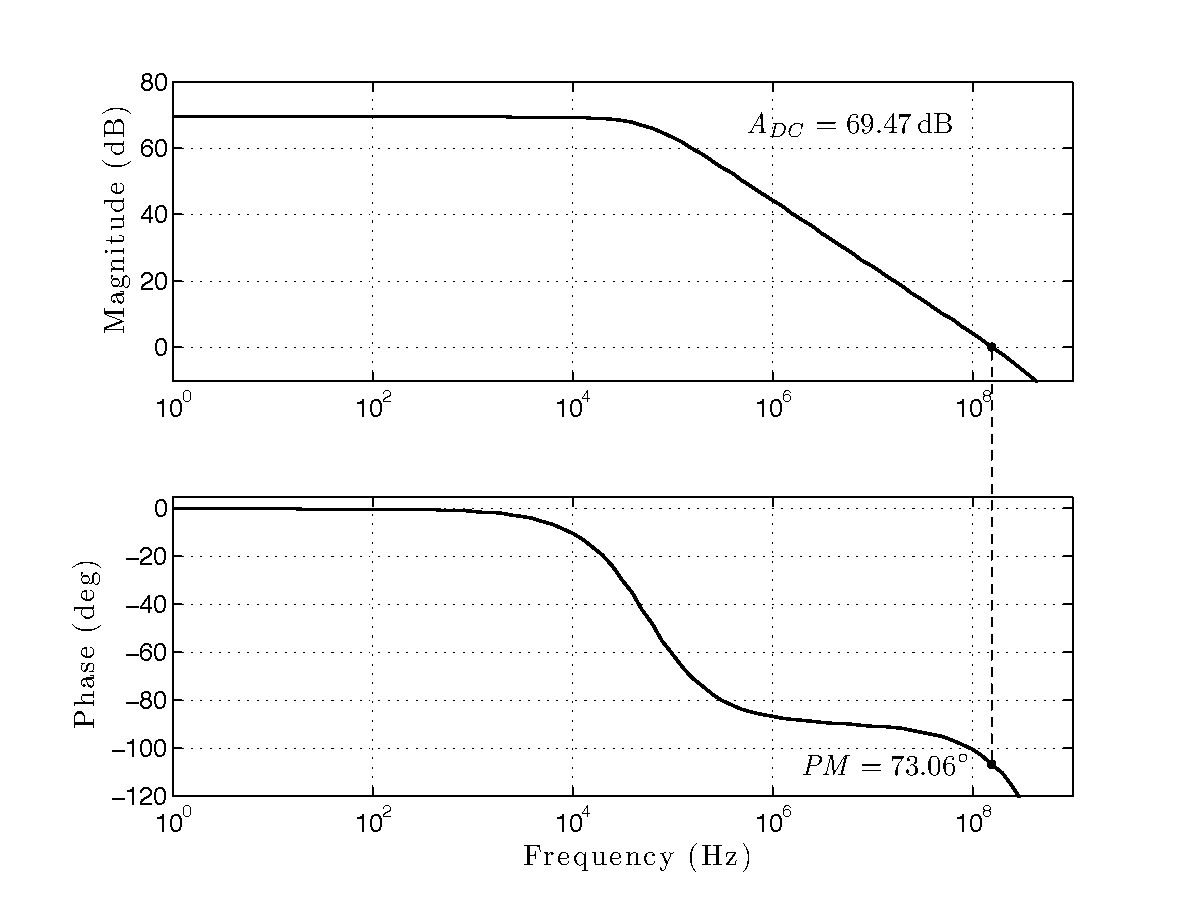
\includegraphics[width=5.3in]{./Test/bode_OTA_post}
	\caption{Bode plot for the OTA open-loop response.}\label{fig:bode_OTA}
\end{figure}


\begin{figure}[!t]
	\centering
	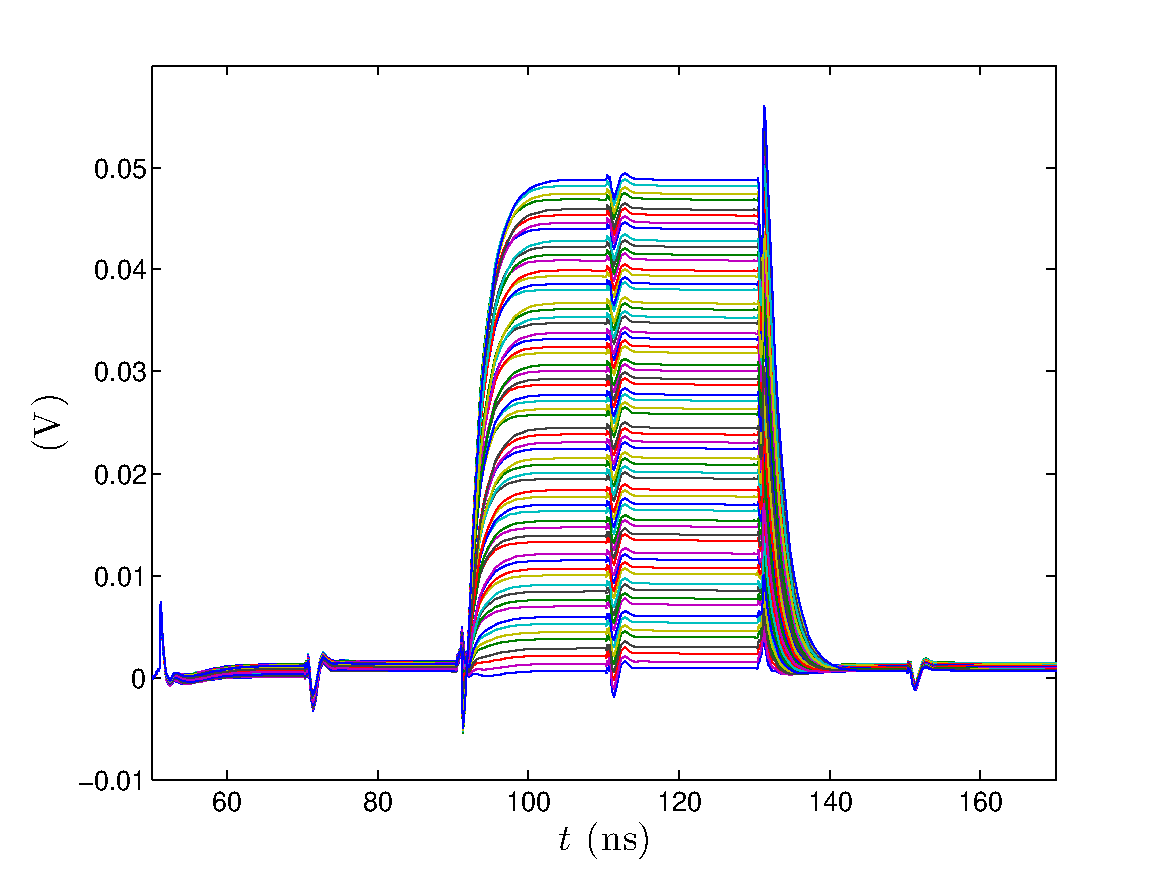
\includegraphics[width=4.4in]{./Test/gain_curves.pdf}
	\caption{Filter output step response with the 64 programmable gains. \mbox{$V_\textit{in}=0.1\,V$} and \mbox{$T_s=40\,\text{ns}$}.}\label{fig:gain_curves}
\end{figure}

\begin{figure}[!t]
	\centering
	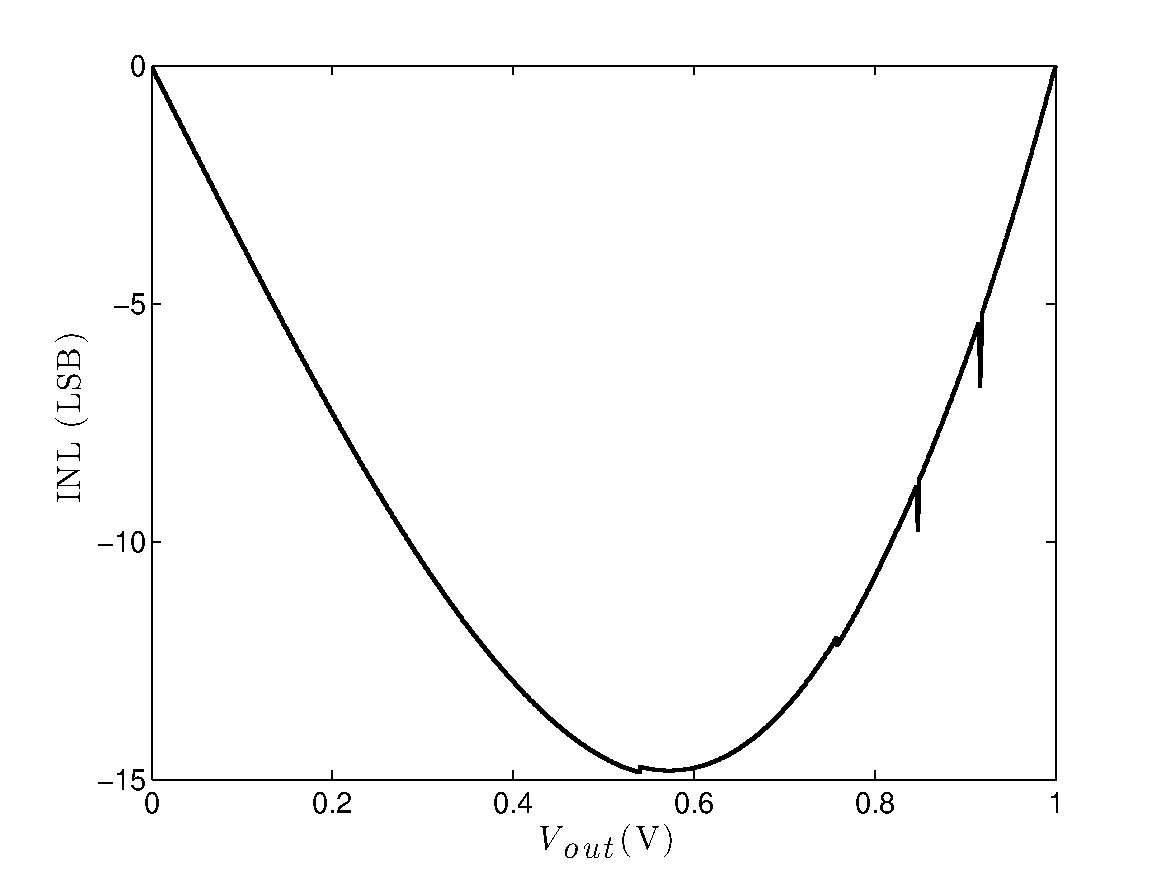
\includegraphics[width=4.4in]{./Test/linearity.pdf}
	\caption{Filter linearity test results, full-scale input range.}\label{fig:gain_curves}
\end{figure}


\begin{figure}[!t]
	\centering
	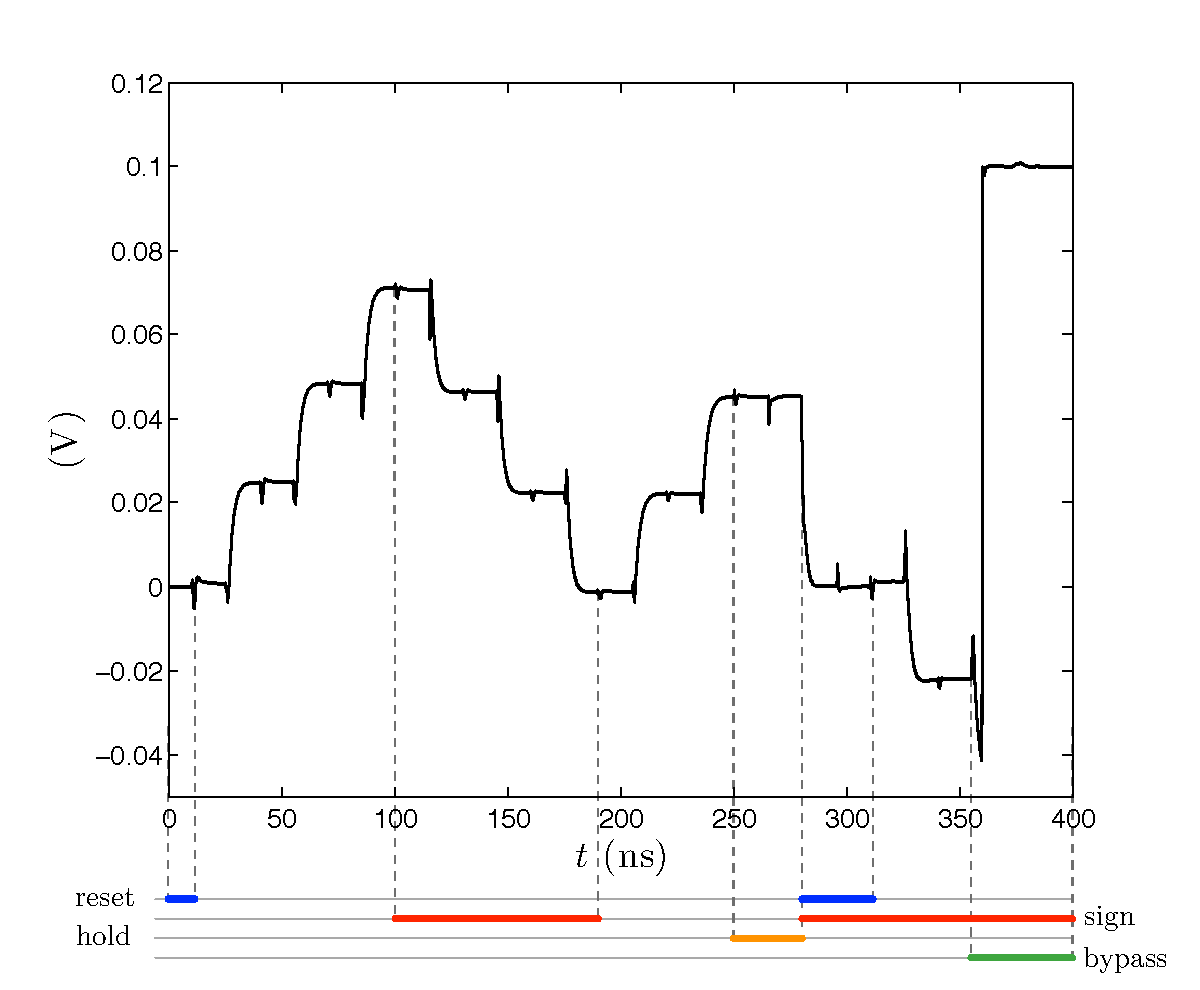
\includegraphics[width=5in]{./Test/test_filter_after_omni.eps}
	\caption{Filter control signals testing. $V_\textit{in}=0.1\,V$ and $\text{gain}=0.25\,V/V$.}\label{fig:test_filter_after_omni}
\end{figure}





\clearpage
\chapter{CONCLUSION}
\label{chapter:conclusion}
\section{Summary}

This thesis deals with the use of discrete-time filters to process the noise present in particle physics detectors front-end circuits. The main contributions of this work are: the development of a new mathematical framework for a design-oriented analysis of \mbox{discrete-time} filters in the \mbox{discrete-time} domain; and the design and implementation of a switched capacitor (SC) filter for arbitrary weighting function (WF) synthesis to be included in the Bean V2 IC.

One of the most important topics in particle physics instrumentation is finding the optimal WF for noise minimization. Although some WFs, such as the cusp \citep{radeka104}, are impossible to synthesize using continuous-time circuits, it was then interesting to determine the fundamental lower limit of noise that could be achieved through them. From then on, design efforts were focused on synthesizing the closest WFs to these theoretical optimal ones. Once introduced the discrete-time pulse shapers in the early 90's, the design efforts remained on this path, by using discrete-time filters to synthesize WFs similar to the continuous-time optimal WFs. However, this approach ignores the discrete-time nature of the pulse shaper, since taking into account this condition results in different optimal WFs, which for a variety of conditions could be very different to the continuos-time counterparts.  This problem leads to the main work presented in this thesis, a mathematical framework to calculate the noise of a typical detector front-end circuit from a \mbox{discrete-time} point of view, and thereby, a powerful tool to design the optimal discrete-time pulse shapers.

From a practical point of view, a generic filter for arbitrary weighting function synthesis is an ideal companion for the theoretical framework mentioned above. The design of this filter was presented in this work, framed on the design of the Bean V2,  an application specific integrated circuit (ASIC) planned to meet the BeamCal instrumentation needs. The use of this filter,  along with a proper characterization of the CSA and detector noise statistics, will allow to minimize the output referred noise on the BeamCal front-end circuit.

\section{Future work}

The mathematical framework presented in this work depends on a proper characterization of the CSA and detector noise statistics to find the optimal filter. Once estimated these parameters, the filter coefficients are computed offline, and then, they are updated in the circuit. An interesting future development could be to find a methodology to compute the filter coefficients online without having to characterize the CSA and detector noise statistics separately. To pursue this problem, the mathematical framework presented in this work represents a proper starting point. Also, given the abstraction of this work, it could find applications in other fields with similar circuit configurations, such as the current developments for astronomical instrumentation \citep{guzman101}.

The lessons learned during the design and simulation of the Bean filter prototype will prompt corrections, improvements, and upgrades for future revisions. Based just on simulation results, the most urgent correction consist of editing the filter OTA design to meet the settling time specification, and thus, the linearity specification.  Filter lab testing are about to start. Additional corrections, improvements, and upgrades are expected as result of this development phase.


% References



%%%%%%%%%%%%%%%%%%%%%%%%%%%%%%%%%%%%%%%%%%%%%%%%%%%%%%%%%%%%%%%%%%%%%%%%
% Begin Appendix

\cleardoublepage
\thispagestyle{empty}
\begin{center}
\vspace*{3.5in}
\large{\bfseries{APPENDIX}}
\addcontentsline{toc}{chapter}{APPENDIX}
\end{center}

\appendix
\cleardoublepage


\chapter{The Bean 2 prototype pinout} 
\label{appendix1}
The Bean V2 prototype has 48 pads and was bonded to a 64-lead package from \mbox{Kyocera} Corporation (KYO). The package KYO part number is QC064307WZ. The Bean V2 bonding diagram is shown in Fig.~\ref{fig:bondpad}.
Table~\ref{tab:pinout} shows the Bean V2 pinout.

\begin{center}
\begin{longtable}{|l|l|l|}\hline
{\bf Pin number} & {\bf Pin name} & {\bf Description} \\ \hline\hline
1 & \verb=AGnd= & Analog ground \\\hline
2 & \verb=AGnd= & Analog ground \\\hline
3 & \verb=AGnd= & Analog ground \\\hline
4 & \verb=NC= & No connection \\\hline
5 & \verb=NC= & No connection \\\hline
6 & \verb=res_bias_ext= & IC bias external resistor \\\hline
7 & \verb=V_ref_prechar= & Reference voltage CSA precharger \\\hline
8 & \verb=NC= & No connection  \\\hline
9 &  \verb=clk_prech1= & CSA precharger clk1  \\\hline
10 & \verb=clk_prech2= & CSA precharger clk2  \\\hline
11 & \verb=NC= & No connection \\\hline
12 & \verb=op_mode= & Operation mode select \\\hline
13 & \verb=rst_csa= & CSA reset  \\\hline
14 & \verb=NC= & No connection \\\hline
15 & \verb=cap_precharge_ext= & CSA precharger external capacitor \\\hline
16 & \verb=Vin_csa= & Vin CSA \\\hline
17 & \verb=NC= & No connection \\\hline
18 & \verb=clk= & IC clock \\\hline
19 & \verb=AGnd= & Analog ground \\\hline
20 & \verb=AGnd= & Analog ground \\\hline
21 & \verb=Vi+_fil= & Filter Vi+ \\\hline
{\bf Pin number} & {\bf Pin name} & {\bf Description} \\ \hline\hline
22 & \verb=Vi-_fil= & Filter Vi- \\\hline
23 & \verb=NC= & No connection \\\hline
24 & \verb=Vo-_bp_fil= & Filter bypass Vo- \\\hline
25 & \verb=Vo+_bp_fil= & Filter bypass Vo+  \\\hline
26 & \verb=NC= & No connection \\\hline
27 & \verb=DVdd= & Digital Vdd \\\hline
28 & \verb=DGnd= & Digital Gnd \\\hline
29 & \verb=NC= & No connection \\\hline
30 & \verb=Vo-_fil= & Filter Vo+ (buffered) \\\hline
31 & \verb=Vo+_fil= & Filter Vo- (buffered) \\\hline
32 & \verb=NC= & No connection \\\hline
33 & \verb=out_s= & Filter output selection \\\hline
34 & \verb=Vocm= & Filter Vocm \\\hline
35 & \verb=hold= & Filter hold signal  \\\hline
36 & \verb=rst= & Filter reset \\\hline
37 & \verb=sgn= & Filter gain sign \\\hline
38 & \verb=Vicm= & Filter Vicm \\\hline
39 & \verb=NC= & No connection \\\hline
40 & \verb=AGnd= & Analog ground \\\hline
41 & \verb=NC= & No connection \\\hline
42 & \verb=NC= & No connection \\\hline
43 & \verb=CS_b0= & Filter CS capacitor bit 0 \\\hline
44 & \verb=CS_b1= & Filter CS capacitor bit 1 \\\hline
45 & \verb=CS_b2= & Filter CS capacitor bit 2 \\\hline
46 & \verb=CS_b3= & Filter CS capacitor bit 3 \\\hline
47 & \verb=CS_b4= & Filter CS capacitor bit 4 \\\hline
{\bf Pin number} & {\bf Pin name} & {\bf Description} \\ \hline\hline
48 & \verb=CS_b5= & Filter CS capacitor bit 5 \\\hline
49 & \verb=AGnd= & Analog ground \\\hline
50 & \verb=AGnd= & Analog ground \\\hline
51 & \verb=Vo+_ch= & Channel Vo+ (buffered) \\\hline
52 & \verb=Vo-_ch= & Channel Vo- (buffered)\\\hline
53 & \verb=NC= & No connection \\\hline
54 & \verb=Vout_csa= & CSA Vout (buffered) \\\hline
55 & \verb=NC= & No connection \\\hline
56 & \verb=baseline= & CSA baseline (buffered) \\\hline
57 & \verb=NC= & No connection \\\hline
58 & \verb=NC= & No connection \\\hline
59 & \verb=NC= & No connection \\\hline
60 & \verb=AGnd= & Analog ground \\\hline
61 & \verb=AGnd= & Analog ground \\\hline
62 & \verb=AGnd= & Analog ground \\\hline
63 & \verb=NC= & No connection \\\hline
64 & \verb=AVdd= & Analog Vdd \\\hline
\caption{The Bean 2 prototype pinout}\label{tab:pinout}
\end{longtable}
\end{center}

\begin{figure}[!t]
	\centering
	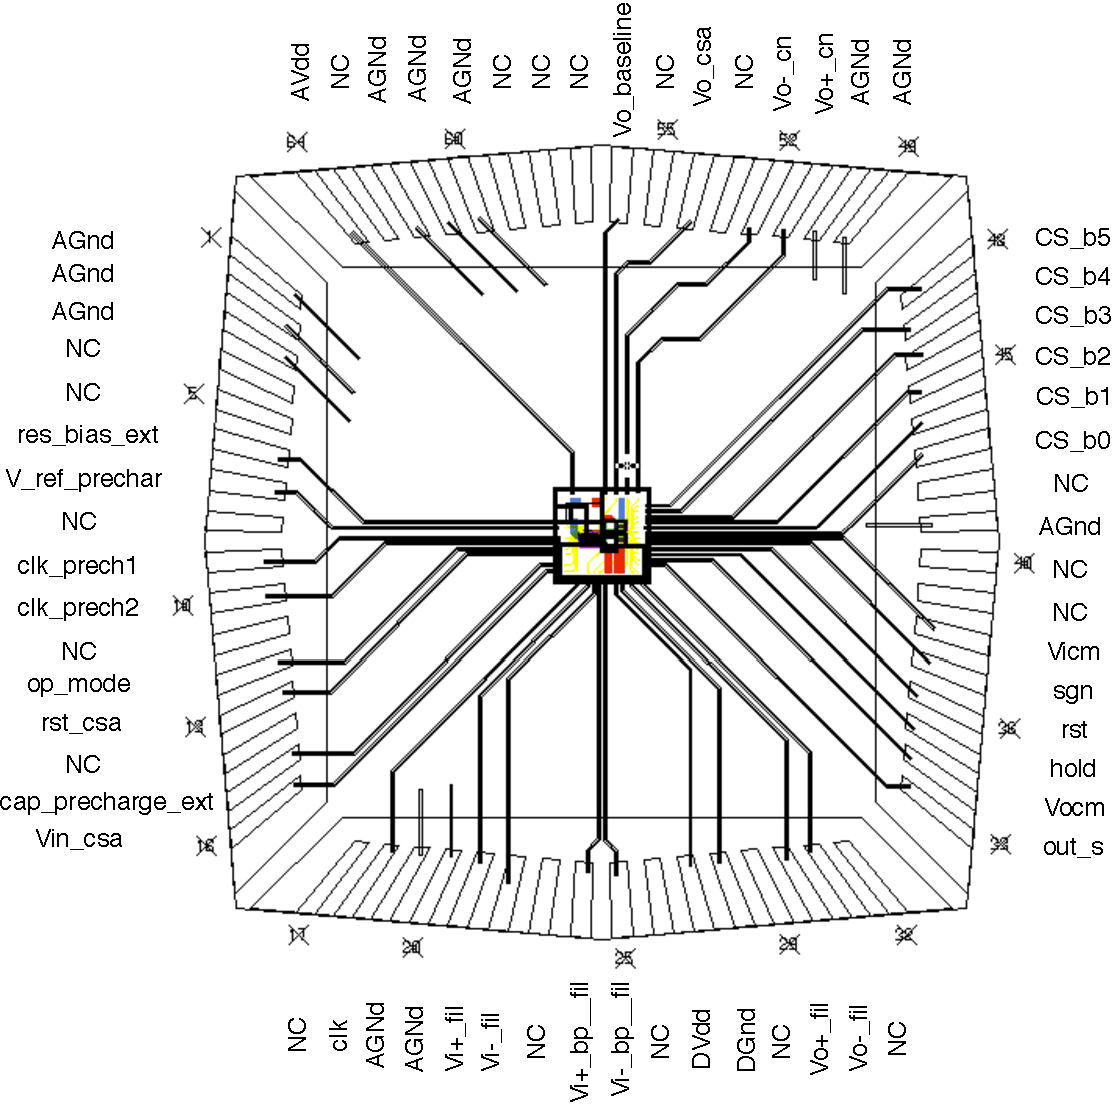
\includegraphics[width=6in]{./Figures/bondpad.pdf}
	\caption{The Bean 2 prototype bonding diagram.}\label{fig:bondpad}
\end{figure}



\cleardoublepage
\bibliographystyle{apacite}
\bibliography{\bibpath/library}
\cleardoublepage

\end{document}


